%% 
%% Journal article based on elsarticle-template-harv.tex
%% Harvard (author-year) bibliographic style
%%

\documentclass[preprint,12pt,authoryear]{elsarticle}

\usepackage{amssymb}
\usepackage{amsmath}
\usepackage{graphicx}
\usepackage{booktabs}
\usepackage{multirow}
\usepackage{array}
\usepackage{subcaption}
\usepackage{xcolor}
\usepackage{colortbl}
\usepackage{placeins}

\journal{Journal of Biomedical Informatics / Computers in Biology and Medicine}

\begin{document}

\begin{frontmatter}

\title{An End-to-End Multimodal Pipeline for Chest X-Ray Disease Classification, Localisation, Lung Segmentation, and Zone-Based Radiology Report Generation}

\author{Aditya Pillai}
\affiliation{organization={Department of Computer Science and Engineering, Indian Institute of Information Technology, Design and Manufacturing (IIITDM) Kancheepuram},
            addressline={},
            city={Chennai},
            postcode={600127},
            state={Tamil Nadu},
            country={India}}

\begin{abstract}
Chest radiography remains one of the most widely used and cost-effective imaging modalities for screening and monitoring thoracic disease, yet its interpretation depends on a limited pool of trained radiologists who must process an ever-growing volume of studies. Existing deep learning systems for chest X-ray (CXR) analysis are typically narrow, black-box, multi-label classifiers that provide no spatial grounding and no clinically structured output, which limits their usefulness as decision-support tools. This work proposes an end-to-end, multimodal pipeline built around an EfficientNet-B3 backbone that (i) performs multi-label classification of 13 thoracic pathologies by fusing image features with patient metadata (age, sex, view position), (ii) localises detected pathologies using a bounding-box regression head trained with a combined CIoU and Smooth-L1 objective, (iii) segments the lung fields using an edge-aware U-Net, and (iv) synthesises the outputs of all three modules into a structured, zone-wise radiology report. The classifier is trained with a multi-label Focal Loss to address severe class imbalance, and per-class decision thresholds are subsequently optimised on a validation set. As an exploratory extension, a short self-supervised pre-training stage inspired by optimal-transport-based representation learning was also evaluated; while it produced a marginal improvement at full label availability, its benefit was inconsistent at lower label fractions and is therefore reported only as a secondary finding. On the NIH ChestX-ray14 dataset, the supervised multimodal classifier achieves a mean AUC-ROC of 0.8636 across 13 disease categories, outperforming ResNet-50 (0.60), DenseNet-121 (0.77), and a ViT/Swin baseline (0.80 after 7 epochs) trained under the same protocol. Per-class threshold optimisation raises the macro-F1 score from 0.3444 to 0.5103. The bounding-box regressor attains a mean IoU of 0.2110 on the NIH BBox\_List\_2017 subset (0.6607 for cardiomegaly), and the edge-aware U-Net achieves a Dice coefficient of 0.9602 and an IoU of 0.9249 for lung-field segmentation on the Shenzhen dataset. These components are combined into a template-driven report generator that attributes detected findings to anatomical zones. The results indicate that a multimodal, modular CNN pipeline offers a practical and explainable route to automated CXR analysis, with auxiliary localisation and segmentation tasks providing the spatial grounding required for structured reporting.
\end{abstract}

\begin{keyword}
Chest X-ray classification \sep Multimodal deep learning \sep EfficientNet \sep Disease localisation \sep Lung segmentation \sep Automated radiology report generation \sep Focal loss
\end{keyword}

\end{frontmatter}

%% ==================================================================
\section{Introduction}
\label{sec:intro}
%% ==================================================================

Chest radiography (chest X-ray, CXR) is one of the most accessible, low-cost, and low-radiation imaging modalities used for the diagnosis and longitudinal monitoring of thoracic diseases such as pneumonia, tuberculosis, pulmonary edema, and lung nodules. Despite its ubiquity, the interpretation of CXRs is a specialist task: radiologists must simultaneously identify the presence of disease, localise the affected anatomical region, and communicate their findings in a structured report. The number of studies generated by modern hospitals, particularly in emergency and tertiary-care settings, has grown far faster than the supply of trained radiologists, producing reporting backlogs that can delay diagnosis and treatment.

Computer-aided diagnosis (CAD) systems based on deep learning, especially convolutional neural networks (CNNs) and, more recently, Vision Transformers, have demonstrated strong performance on multi-label CXR classification benchmarks. However, three limitations recur across the literature and in practice. First, most systems operate as \emph{black-box classifiers} that output disease probabilities without any spatial evidence, which limits clinician trust. Second, very few systems integrate \emph{patient-level context} (age, sex, view position, clinical history) despite radiologists routinely using such context during interpretation. Third, classification, localisation, segmentation, and report generation are usually studied as separate problems on separate datasets, with little work demonstrating how they can be combined into a single, coherent, end-to-end pipeline that produces a clinically structured output.

The strategy adopted in this work is predominantly \emph{supervised}: a multimodal EfficientNet-B3 classifier is trained on multi-hot disease labels together with patient metadata using a multi-label Focal Loss; a bounding-box regression head is trained on a smaller set of expert-annotated boxes using a combined CIoU and Smooth-L1 loss; and an edge-aware U-Net is trained on binary lung masks using a combination of Dice, boundary-weighted binary cross-entropy, and an auxiliary edge-prediction loss. In addition, a short \emph{self-supervised} pre-training stage inspired by optimal-transport (OT) based alignment of augmented views was explored as an optional initialisation step for the classification backbone. As discussed in Section~\ref{sec:results}, this self-supervised stage produced only a marginal change in overall performance and degraded label efficiency at lower label fractions; it is therefore reported as an exploratory secondary contribution rather than a central claim of this work.

\subsection{Existing Approaches}
\label{sec:existing}

Recent work on automated CXR reporting can be broadly grouped into three families. \emph{Multimodal alignment approaches} attempt to learn a shared embedding space between image features, textual report representations, and disease labels, either by learning a knowledge base end-to-end \citep{yang_knowledge} or by fusing multi-scale visual features with patient history encoded through pretrained language models \citep{mmg_fusion}. \emph{Modular pipeline approaches} decompose the report-generation task into interpretable stages classification, Grad-CAM-based visual explanation, anatomical segmentation, and template-based language generation so that each stage can be validated independently \citep{ihras}. \emph{Retrieval-augmented and concept-based approaches} either retrieve similar historical cases to anchor generation in real clinical examples \citep{xrem}, or first predict an interpretable set of medical concepts and then use a retrieval-augmented generation (RAG) agent to produce the final report \citep{concept_rag}. Broader surveys of the field highlight the continued importance of structured clinical context \citep{integrative_multimodal}, explainability \citep{xai_survey}, and the rapid pace of new architectures being proposed for this task \citep{pmc_advancements,awesome_rrg}.

\subsection{Gaps in Existing Approaches}
\label{sec:gaps}

Despite this progress, several gaps remain. Knowledge-base alignment methods \citep{yang_knowledge} improve language-generation metrics (BLEU, ROUGE) but provide no pixel- or region-level grounding, and the learned knowledge base is itself difficult to interpret. Methods that incorporate structured clinical context \citep{integrative_multimodal} mimic clinical reasoning but are sensitive to missing or noisy structured fields and risk confirmation bias toward symptom-driven predictions. Multi-granularity fusion methods \citep{mmg_fusion} improve detection of subtle findings but increase architectural complexity and reduce interpretability because multiple feature scales are fused before the decision layer. Modular pipelines such as IHRAS \citep{ihras} are transparent and stage-wise validated, but errors in early stages (e.g.\ classification) cascade into later stages (segmentation, report text) without a mechanism for correction. Retrieval-based methods \citep{xrem} reduce hallucination but depend heavily on the coverage and quality of the retrieval corpus, and concept-bottleneck RAG systems \citep{concept_rag} add substantial computational overhead. Across all of these families, very few systems jointly (a) fuse imaging with patient metadata, (b) localise findings with bounding boxes, (c) segment anatomical lung fields, and (d) synthesise a zone-attributed structured report, all within a single pipeline evaluated on a large public dataset.

\subsection{Contributions of this Work}
\label{sec:contributions}

The contributions of this paper are as follows:
\begin{enumerate}
    \item A \textbf{multimodal multi-label classifier} based on EfficientNet-B3 that fuses image features with patient age, sex, and view-position metadata, trained with a multi-label Focal Loss to address the severe class imbalance present in the NIH ChestX-ray14 dataset, together with per-class threshold optimisation that substantially improves macro- and micro-F1.
    \item A \textbf{disease localisation module} that reuses the classification backbone and adds a disease-conditioned bounding-box regression head trained with a combined CIoU and Smooth-L1 loss, evaluated on the NIH BBox\_List\_2017 annotation subset.
    \item An \textbf{edge-aware U-Net} for lung-field segmentation trained on the Shenzhen Chest X-ray dataset, combining Dice loss, boundary-weighted binary cross-entropy, and an auxiliary edge-prediction head.
    \item A \textbf{zone-based, template-driven radiology report generator} that combines the outputs of the three modules above: segmented lung fields are divided into six anatomical zones (upper/middle/lower, left/right), detected pathologies are attributed to the zone of maximum bounding-box overlap, and a structured report (patient information, findings summary, zonal analysis, and impression) is produced automatically.
    \item An \textbf{exploratory evaluation} of optimal-transport-inspired self-supervised pre-training as an optional initialisation strategy, reported transparently including the regimes in which it does and does not help.
\end{enumerate}

\subsection{Organisation of the Paper}
\label{sec:organisation}

The remainder of this paper is organised as follows. Section~\ref{sec:litreview} reviews recent literature on automated chest X-ray reporting and identifies the positioning of this work relative to existing approaches. Section~\ref{sec:methodology} describes the proposed pipeline, including the dataset, preprocessing and augmentation strategies, the architecture of each module, and the loss functions used for training. Section~\ref{sec:results} presents the experimental results for classification, threshold optimisation, localisation, and segmentation, together with an analysis of the self-supervised pre-training experiment. Section~\ref{sec:comparison} compares the proposed approach against supervised baselines and contextualises the results relative to the broader literature. Section~\ref{sec:conclusion} concludes the paper and outlines directions for future work.

%% ==================================================================
\section{Literature Review}
\label{sec:litreview}
%% ==================================================================

This section reviews recent (2021--2026) work on deep-learning-based chest X-ray analysis and automated radiology report generation, organised by methodological family.

\subsection{Knowledge- and Multimodal-Alignment Approaches}

\citet{yang_knowledge} proposed a radiology report generation framework that learns a medical knowledge base \emph{during} training rather than relying on a predefined knowledge graph. The model jointly aligns image features, textual report representations, and disease-label embeddings in a shared embedding space, allowing the network to discover semantic relationships between anatomical structures and clinical phrases without manual ontology engineering. Evaluated on the IU-XRAY and MIMIC-CXR datasets, the approach reported improvements in BLEU and ROUGE scores relative to earlier captioning-style baselines. The principal limitation is that the learned knowledge base is opaque clinicians cannot inspect what relationships the model has encoded -- and the method provides no region- or pixel-level grounding of its findings, which is precisely the gap that the localisation and segmentation modules in this work aim to address.

\citet{mmg_fusion} proposed a multi-granularity feature-fusion architecture for chest X-ray report generation, combining multi-scale image features extracted with a Swin Transformer, disease-label embeddings, patient-history embeddings produced by BioBERT, and a DistilGPT2 language decoder. By fusing global and local visual features, the model is better able to detect both large, diffuse abnormalities (e.g.\ pleural effusion) and small, localised findings (e.g.\ nodules). This design motivates the present work's choice of an EfficientNet-B3 backbone, which similarly produces rich multi-scale feature maps, and its use of patient metadata as an auxiliary input stream, although in a simpler tabular (rather than free-text history) form.

\subsection{Structured Clinical Context}

\citet{integrative_multimodal} argue that radiologists rarely interpret a chest X-ray in isolation: vital signs, presenting symptoms, and patient history materially change the differential diagnosis. Their approach incorporates such structured clinical information through a cross-attention mechanism that learns to weight different modalities while generating the report. While this more closely mirrors clinical reasoning, the authors note two risks: confirmation bias, where the model over-relies on symptom text rather than image evidence, and brittleness to missing or inconsistent structured fields. The present work adopts a conservative version of this idea fusing only three reliably available metadata fields (age, sex, view position) -- which avoids the missing-data problem while still allowing the classifier to condition its predictions on patient context.

\subsection{Modular, Component-Based Pipelines}

\citet{ihras} describe a modular pipeline (referred to as IHRAS) that decomposes automated reporting into multi-label disease classification, Grad-CAM-based visual explanation, anatomical segmentation, and structured language generation. Because each stage can be independently validated, the pipeline is transparent: segmentation outputs provide anatomical grounding, and Grad-CAM visualisations let a radiologist verify whether the model attended to clinically relevant regions. The principal weakness of modular pipelines of this kind is error cascading a mistake in an early stage (e.g.\ a missed classification) propagates to later stages without correction. The pipeline proposed in this work follows the same modular philosophy (classification, localisation, segmentation, report generation) but additionally couples the localisation and segmentation outputs directly through the zone-attribution step, so that the spatial evidence used in the final report is derived from two independently trained but jointly consulted modules.

\subsection{Retrieval-Augmented and Concept-Based Approaches}

\citet{xrem} proposed a multimodal retrieval-based generation approach that retrieves historically similar cases from a large corpus to anchor the generated report in real clinical examples, improving factual consistency, particularly for rare conditions. The main limitation is that performance depends heavily on retrieval accuracy and on the coverage of the underlying corpus for novel presentations. \citet{concept_rag} extend this idea by first predicting an explicit, human-interpretable set of medical concepts (e.g.\ cardiomegaly, effusion) as a concept bottleneck, then using a multi-agent RAG system to retrieve supporting evidence and generate the final report. This design allows clinicians to correct concept predictions before generation, supporting human-in-the-loop validation, but at the cost of substantially increased system complexity. Both approaches are complementary to the present work: the structured findings summary and per-zone confidence scores produced by the proposed pipeline could, in principle, serve as the concept bottleneck or retrieval query for such systems.

\subsection{Explainability and Survey Perspectives}

\citet{xai_survey} survey explainability techniques for automated CXR report generation, emphasising the need for quantitatively validated explanations rather than purely qualitative saliency maps. \citet{pmc_advancements} provide a broader review of recent advances in radiology report generation, situating knowledge-alignment, retrieval, and concept-based methods within a common taxonomy, and a community-maintained survey of recent literature is also tracked in \citet{awesome_rrg}. These reviews motivate the design choice in this work to favour \emph{quantitatively measurable} spatial grounding bounding-box IoU and segmentation Dice/IoU over purely visual explanation techniques such as saliency maps.

\subsection{Positioning of this Work}

% \noindent\textit{Note to authors / reviewers:} two entries currently in the bibliography (\texttt{miccai2024\_paper2185} and \texttt{miccai2025\_paper3102}) are placeholders with incomplete author/title metadata and should be replaced with the intended MICCAI 2024/2025 references (e.g.\ on radiology lexicon construction or structural alignment) before submission. Similarly, the \texttt{ihras} and \texttt{xai\_survey} entries currently share an identical volume/issue/page range (vol.~12, no.~22, p.~11750) despite different titles and journals, which should be corrected to the correct bibliographic details for each source.
% 
Relative to the approaches reviewed above, this work differs in three respects. First, rather than targeting free-text report quality (BLEU/ROUGE) directly, it targets the three measurable sub-tasks -- multi-label classification, bounding-box localisation, and lung segmentation -- that together provide the evidence a structured report should be built upon. Second, it fuses imaging with a small, reliably available set of patient metadata rather than free-text clinical history, avoiding the missing-data and confirmation-bias risks identified by \citet{integrative_multimodal}. Third, it explicitly couples the segmentation and localisation outputs through a zone-division step to produce a zone-attributed structured report, in the spirit of -- but more tightly integrated than -- the modular IHRAS pipeline \citep{ihras}.

%% ==================================================================
\section{Methodology}
\label{sec:methodology}
%% ==================================================================

\subsection{Overview}

The proposed pipeline consists of four stages: (i) a multimodal multi-label classifier that fuses chest X-ray image features with patient metadata; (ii) a disease-conditioned bounding-box regressor for localisation; (iii) an edge-aware U-Net for lung-field segmentation; and (iv) a post-processing stage that divides the segmented lung fields into six anatomical zones, attributes each detected pathology to a zone, and synthesises a structured radiology report. An optional, exploratory self-supervised pre-training stage for the classification backbone is also described, although -- as discussed in Section~\ref{sec:results} its contribution to the final results is modest. Figure~\ref{fig:architecture} illustrates the overall system architecture.
\FloatBarrier
\begin{figure}[ht]
    \centering
    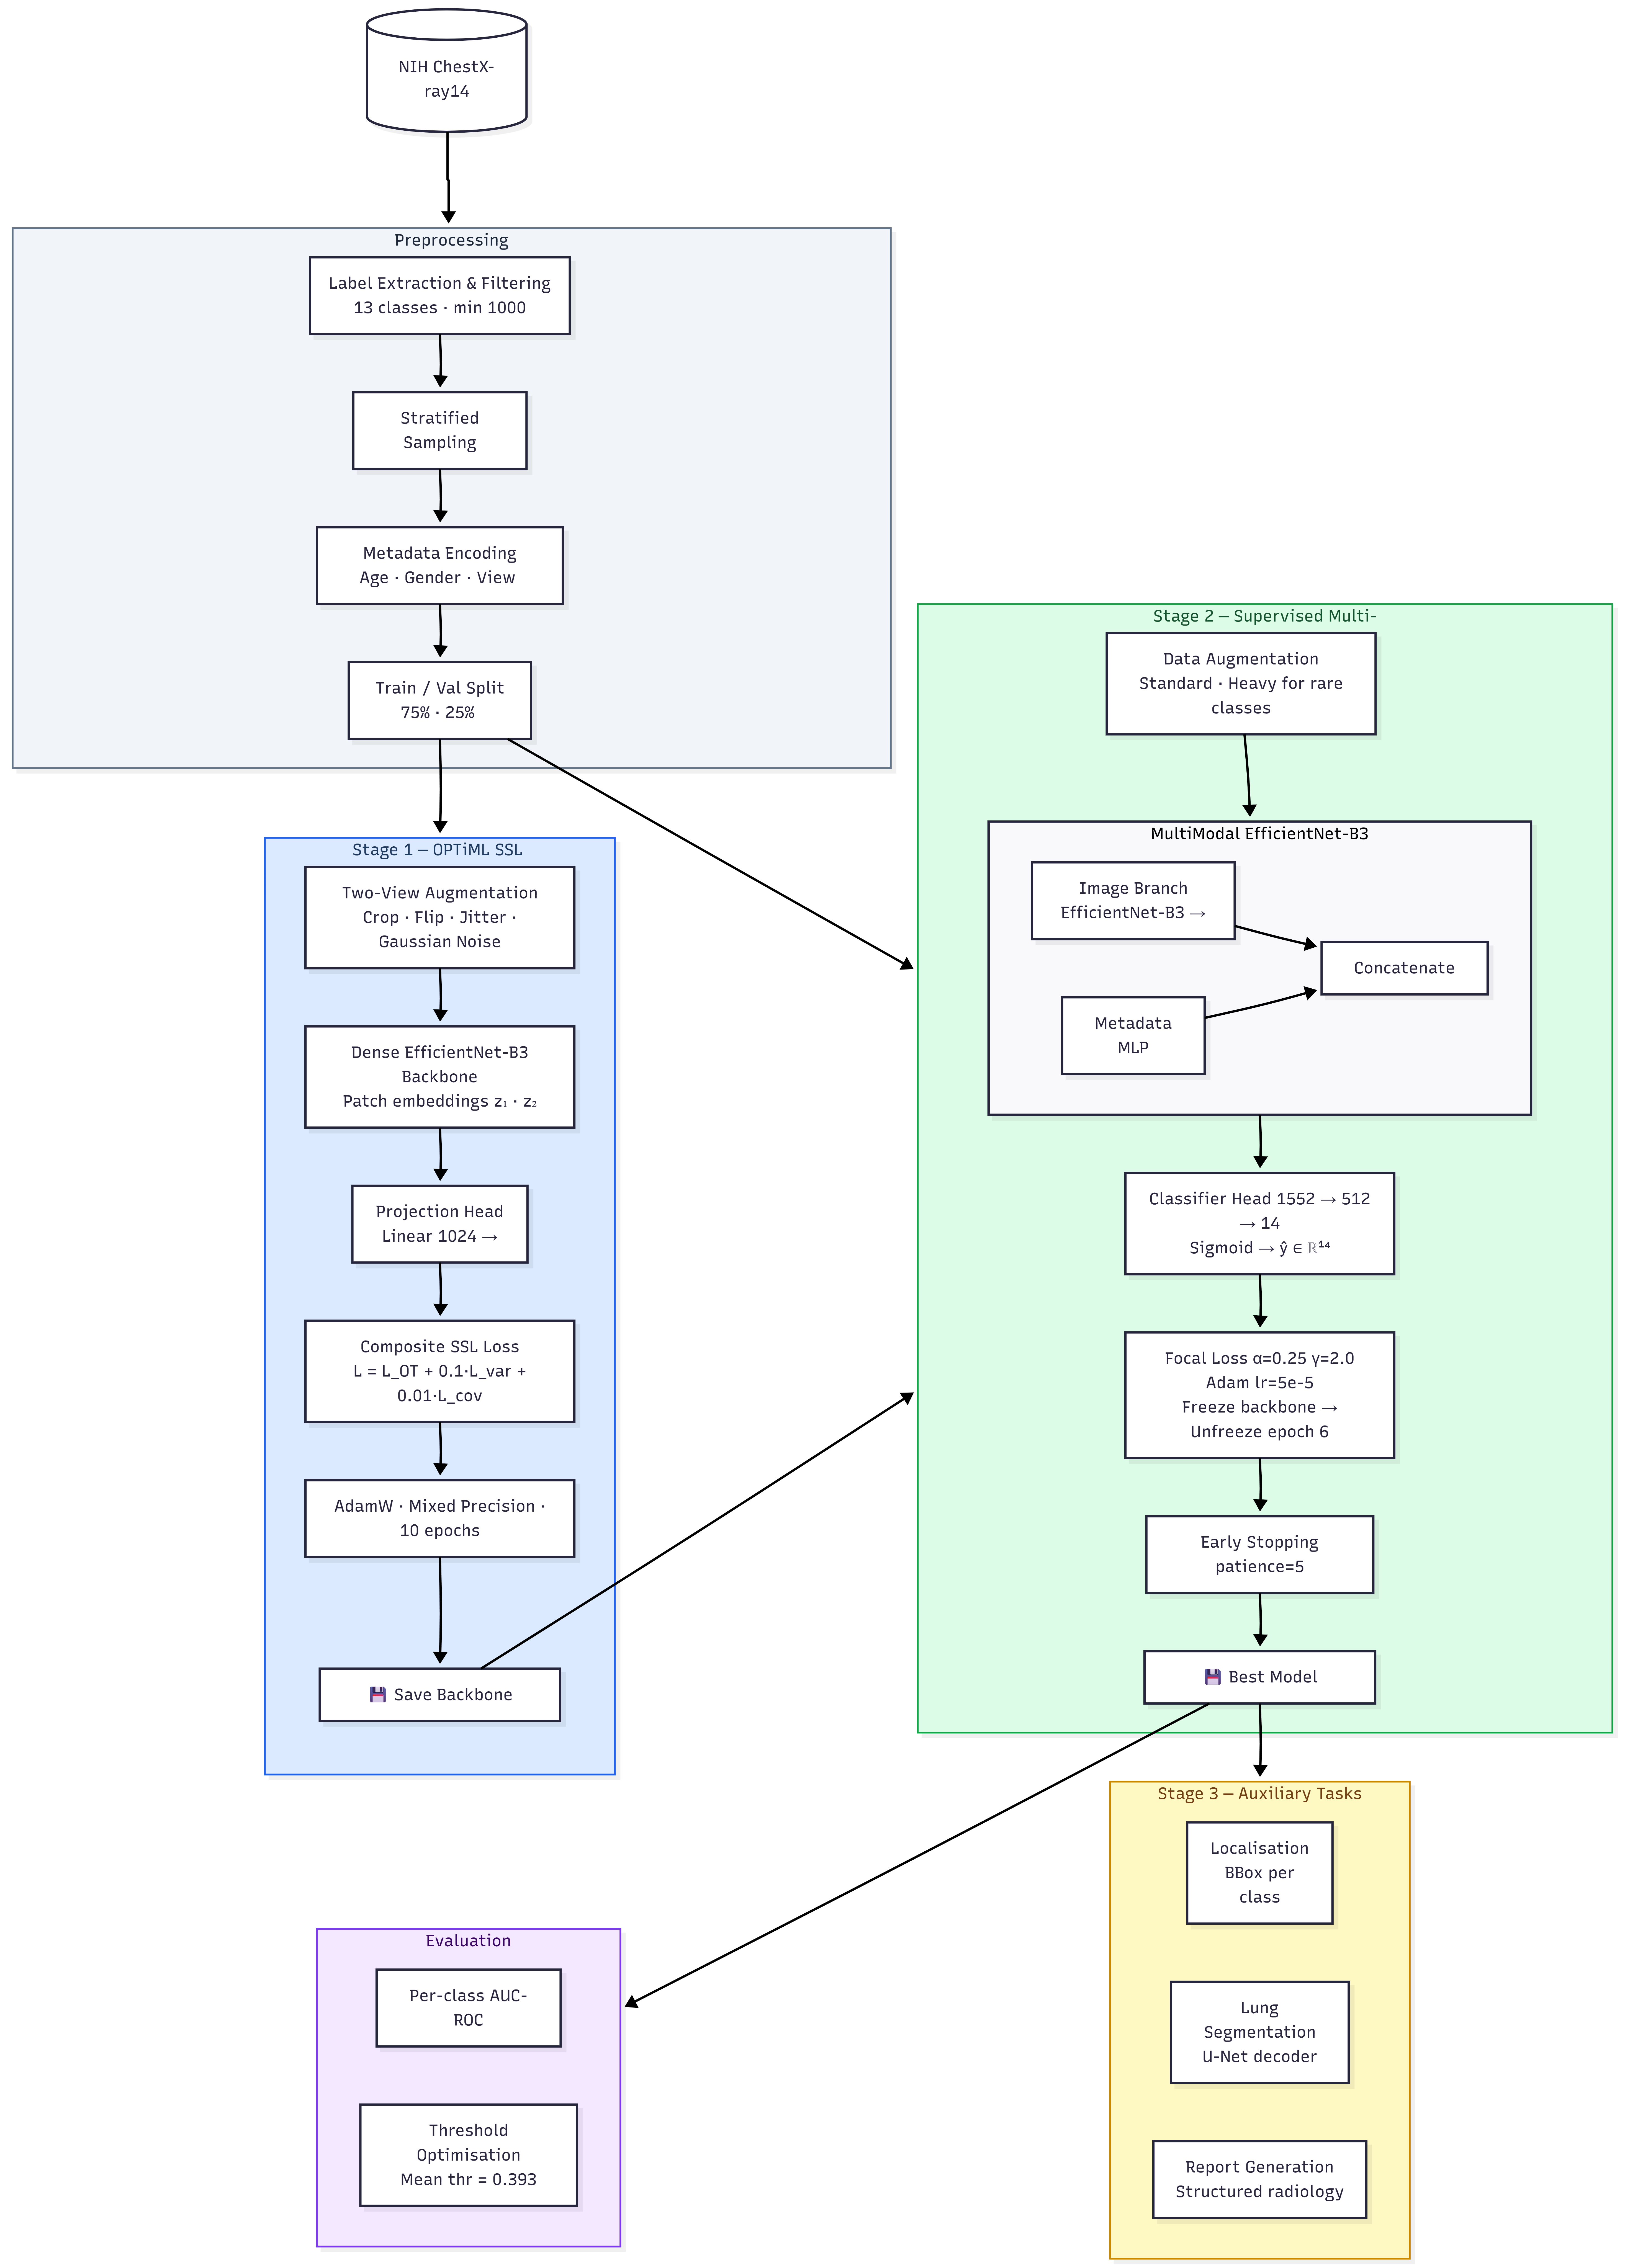
\includegraphics[width=\textwidth]{architecture_flow.png}
    
    \label{fig:architecture}
\end{figure}
\FloatBarrier
\subsection{Dataset}
\label{sec:dataset}

\subsubsection{NIH ChestX-ray14}

The classification and localisation experiments use the NIH ChestX-ray14 dataset, one of the largest publicly available collections of frontal chest radiographs, containing over 100{,}000 images from more than 30{,}000 unique patients with 14 disease labels mined from radiology reports via natural language processing. Labels occurring in fewer than 1{,}000 images were excluded to ensure statistical reliability, leaving 13 disease categories. To address severe class imbalance, a stratified sampling strategy capped the number of samples per class at 10{,}000 during training set construction, preventing any single disease from dominating the training distribution.

For disease localisation, the NIH \texttt{BBox\_List\_2017.csv} file provides expert-annotated pixel-coordinate bounding boxes for 880 images spanning 8 disease categories, with coordinates $(x, y, w, h)$ relative to the original $1024 \times 1024$ image resolution. Patient metadata is joined from \texttt{Data\_Entry\_2017.csv} using the image filename, with median-value imputation for any missing entries, and the localisation data is split 80/20 with stratification on disease label.

\subsubsection{Shenzhen Chest X-ray Dataset}

Lung segmentation is trained on the Shenzhen Chest X-ray dataset, which provides frontal radiographs with expert-delineated binary lung masks. Training is restricted to normal (non-tuberculosis) cases to avoid confounding mask quality with pathology-related structural changes, using an 85/15 train/validation split. Masks are matched to images by filename, with mask filenames suffixed by \texttt{\_mask}.

\subsection{Preprocessing and Augmentation}
\label{sec:preprocessing}

All images are loaded as RGB and resized to a fixed resolution; patient age is clipped to $[0, 100]$ and divided by 100, while sex and view position (PA/AP) are numerically encoded. Multi-hot label encoding maps each finding string to a binary vector of length equal to the number of disease classes. Two augmentation pipelines are used depending on class frequency: a standard pipeline (resize, random horizontal flip, normalisation) for common classes, and a heavier pipeline -- adding random rotation ($\pm20^{\circ}$), random resized crop (zoom 0.8--1.0), random affine translation (10\%), and colour jitter -- for rare classes such as Hernia, Fibrosis, and Emphysema.

For bounding-box regression, geometric augmentations are deliberately \emph{removed}, since operations such as flipping, rotation, and cropping move pixels without updating the target coordinates and would corrupt the supervision signal; only photometric transforms (resize to $448\times448$, colour jitter, normalisation) are retained. For segmentation, joint augmentations that preserve image--mask correspondence are used: horizontal flip, small-angle rotation ($\pm10^{\circ}$), and brightness/contrast jitter, followed by resizing to $512\times512$ and normalisation with mean $0.5$ and standard deviation $0.5$.

All RGB inputs to the EfficientNet-B3-based modules are normalised using ImageNet statistics ($\mu = [0.485, 0.456, 0.406]$, $\sigma = [0.229, 0.224, 0.225]$) to align with the pretrained backbone weights; the segmentation U-Net, trained from scratch on single-channel inputs, uses mean/standard deviation of $0.5$.

\subsection{Multimodal Classification Architecture}
\label{sec:classifier-arch}

The classifier is a multimodal EfficientNet-B3 model with three components. The \emph{image branch} is an EfficientNet-B3 backbone, initialised from ImageNet-pretrained weights with its classification head replaced by an identity mapping, producing a feature vector $\mathbf{z}_{img} \in \mathbb{R}^{1536}$. The \emph{metadata branch} is a two-layer multilayer perceptron (Linear$(3\rightarrow16)$, ReLU, Dropout) that maps the three-dimensional metadata vector (age, sex, view position) to $\mathbf{z}_{meta} \in \mathbb{R}^{16}$. The \emph{fusion classifier head} concatenates $[\mathbf{z}_{img}, \mathbf{z}_{meta}] \in \mathbb{R}^{1552}$ and passes it through a fully connected layer (Linear$(1552\rightarrow512)$, ReLU, Dropout) followed by an output layer Linear$(512\rightarrow13)$ that produces per-class disease logits. The model has approximately 10.5\,M total parameters; a progressive unfreezing schedule keeps the backbone frozen for the first five epochs (training only the head, $\sim$802\,K parameters) before unfreezing the full network at epoch~6 with a reduced learning rate of $10^{-5}$.

\subsection{Optional Self-Supervised Pre-Training (Exploratory)}
\label{sec:ssl}

As an exploratory extension, a dense EfficientNet-B3 backbone (producing spatial feature maps rather than a globally pooled vector) was pre-trained for three epochs without disease labels, using a composite loss inspired by optimal-transport-based self-supervised alignment \citep{otcxr} and informed more generally by the contrastive and redundancy-reduction principles of \citet{simclr} and \citet{barlow_twins}. Two augmented views of each image are aligned via a Sinkhorn-regularised optimal-transport plan over patch embeddings, combined with variance and covariance regularisation terms that discourage representation collapse (Section~\ref{sec:loss-ssl}). The resulting backbone was then used to initialise the supervised classifier described in Section~\ref{sec:classifier-arch}. As shown in Section~\ref{sec:results}, this initialisation gave only a marginal improvement in mean AUC-ROC at full label availability and did not consistently improve label efficiency at reduced label fractions; it is reported here for completeness rather than as a core component of the proposed pipeline.

\subsection{Disease Localisation: Multimodal Bounding-Box Regressor}
\label{sec:bbox-arch}

The localisation module reuses the EfficientNet-B3 image branch (with weights initialised from the trained classifier) and the same metadata branch, and adds a \emph{disease-label branch}: a small MLP that maps a one-hot disease vector $\mathbf{y}_{oh} \in \{0,1\}^{13}$ to $\mathbf{z}_{label} \in \mathbb{R}^{32}$, allowing a single model to localise any of the 13 disease classes by conditioning on the disease of interest. The concatenated features $[\mathbf{z}_{img}, \mathbf{z}_{meta}, \mathbf{z}_{label}] \in \mathbb{R}^{1584}$ pass through a four-layer regression head (Linear$(1584\rightarrow512)$, LayerNorm, GELU, Dropout(0.4); Linear$(512\rightarrow256)$, LayerNorm, GELU, Dropout(0.3); Linear$(256\rightarrow128)$, GELU, Dropout(0.2); Linear$(128\rightarrow4)$, Sigmoid), producing a predicted box $\hat{\mathbf{b}} = (\hat{c}_x, \hat{c}_y, \hat{w}, \hat{h}) \in [0,1]^4$ in centre-form coordinates. Ground-truth boxes $(x, y, w, h)$ are converted to centre form and normalised by image width $W$ and height $H$:
\begin{equation}
c_x = \frac{x}{W} + \frac{w}{2W}, \qquad c_y = \frac{y}{H} + \frac{h}{2H}, \qquad \hat{w} = \frac{w}{W}, \qquad \hat{h} = \frac{h}{H}.
\end{equation}
All predicted coordinates are clamped to $[0,1]$ to prevent out-of-image predictions.

\subsection{Lung Segmentation: Edge-Aware U-Net}
\label{sec:unet-arch}

The segmentation model is a five-level U-Net operating on single-channel $512\times512$ inputs, with four encoder stages (max-pooling downsampling), a bottleneck, and four symmetric decoder stages with bilinear upsampling and skip connections, all convolutions implemented as DoubleConv blocks (two Conv--BatchNorm--ReLU layers). The key architectural addition is an \emph{edge head}: a $1\times1$ convolution applied to the final decoder feature map that predicts a binary boundary-probability map alongside the main segmentation mask,
\begin{equation}
\hat{M}, \hat{E} = f_\theta(X), \qquad \hat{M}, \hat{E} \in [0,1]^{H\times W},
\end{equation}
where $\hat{M}$ is the predicted lung-mask probability and $\hat{E}$ is the predicted edge map. This multi-task formulation gives the decoder explicit gradient signal at lung boundaries, which are both the most clinically significant and the most difficult region to segment precisely. Figure~\ref{fig:unet_arch} shows the architecture.
\FloatBarrier
\begin{figure}[p]
    \centering
    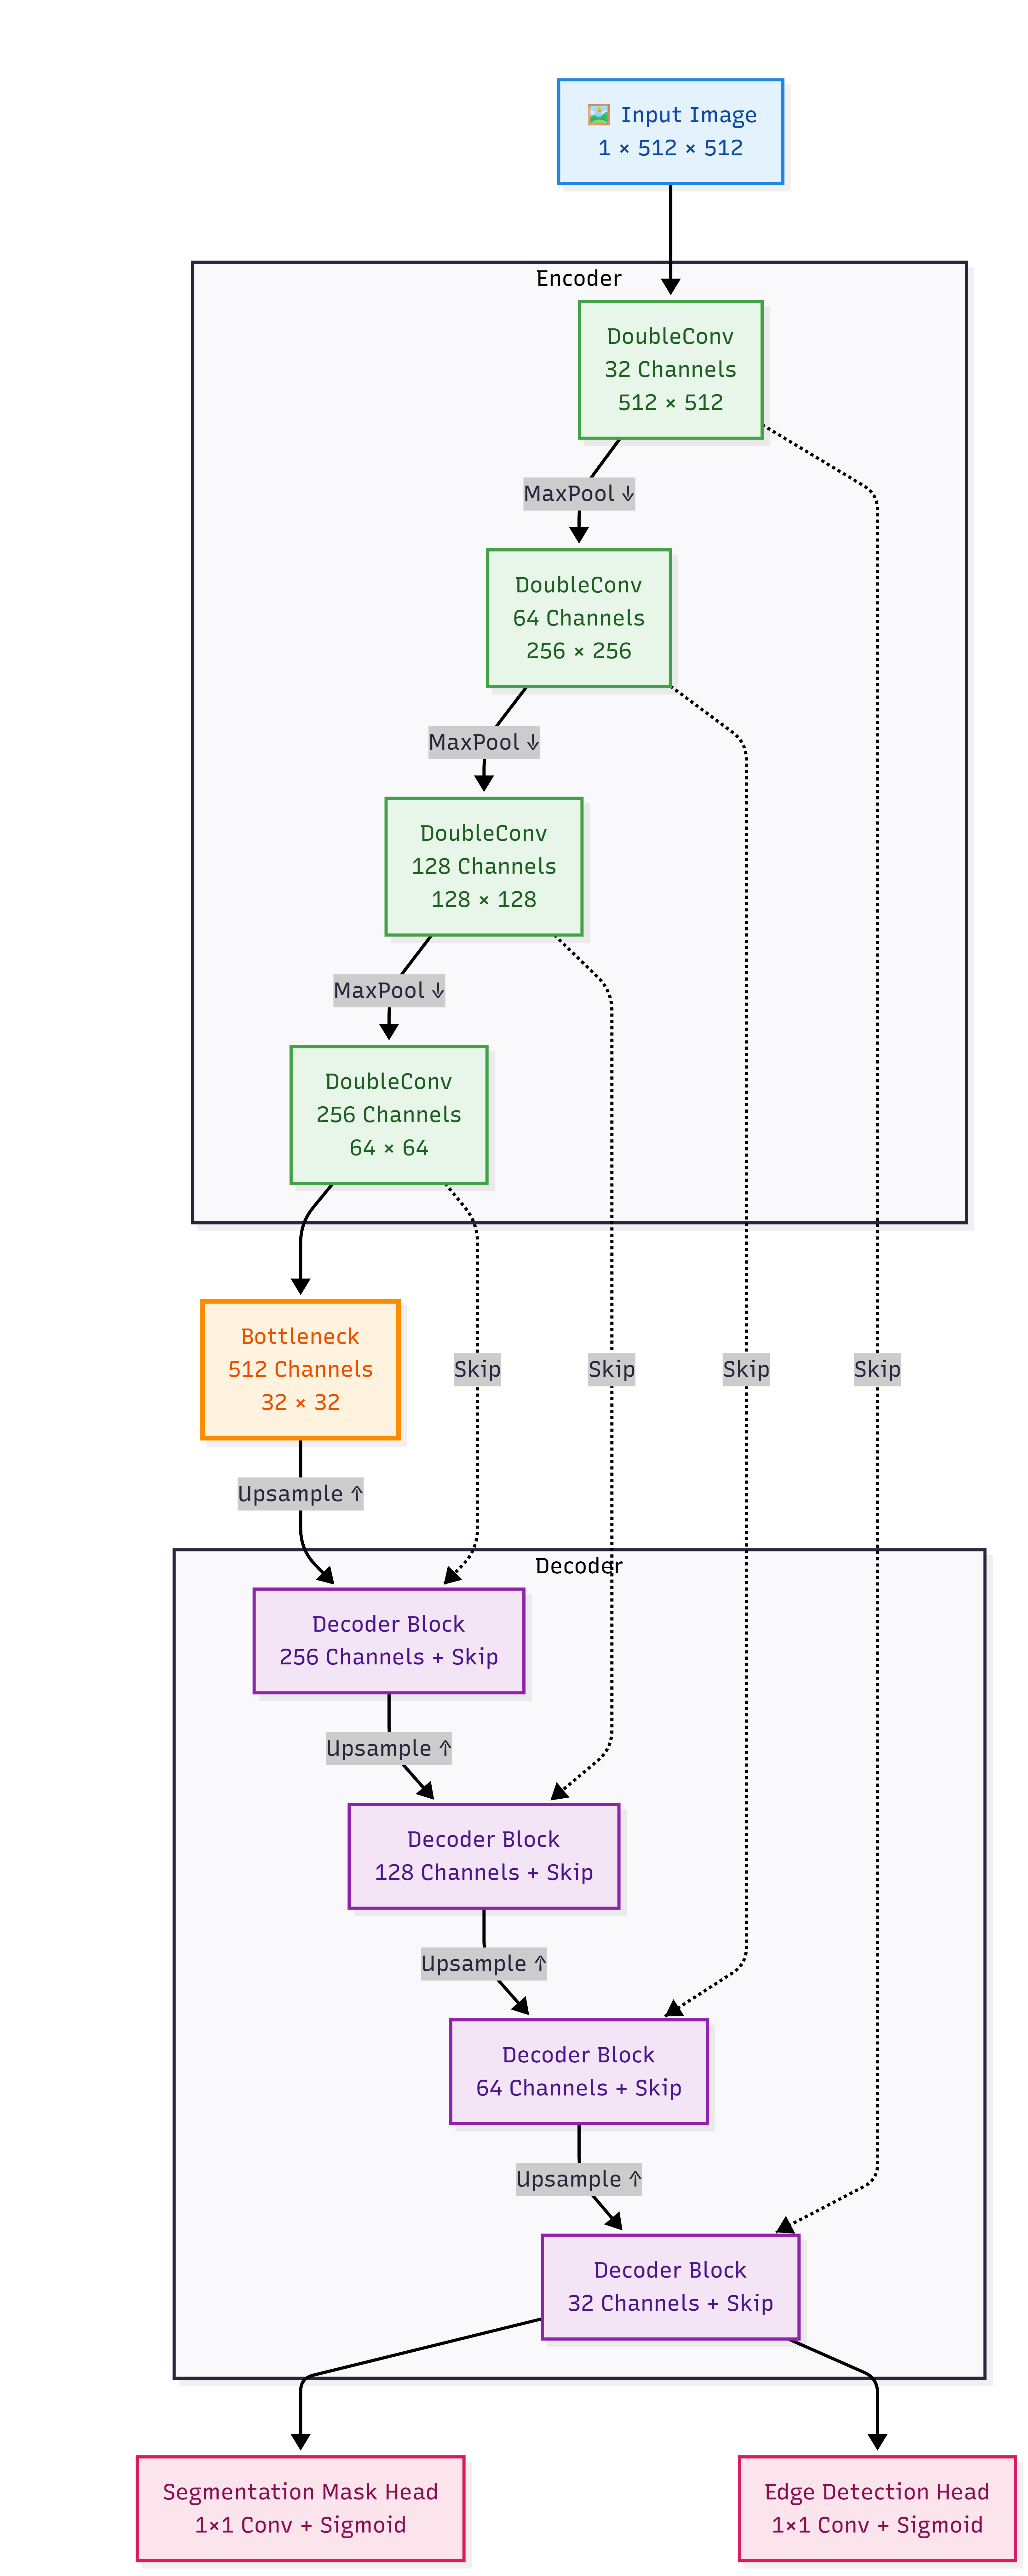
\includegraphics[
        width=\textwidth,
        height=0.92\textheight,
        keepaspectratio
    ]{unetarchitecture.png}
    \caption{Edge-Aware U-Net for lung segmentation with dual mask and edge output heads.}
    \label{fig:unet_arch}
\end{figure}
\FloatBarrier
\subsection{Loss Functions}
\label{sec:losses}

\subsubsection{Multi-Label Focal Loss}

Given the severe class imbalance of the NIH ChestX-ray14 dataset, the classifier is trained with a multi-label Focal Loss rather than standard binary cross-entropy:
\begin{equation}
\mathcal{L}_{\text{Focal}} = -\alpha \sum_{i} (1-p_t)^{\gamma}\,\text{BCE}(\hat{y}_i, y_i),
\end{equation}
where $p_t = \sigma(\hat{y}_i)$ if $y_i=1$ and $p_t = 1-\sigma(\hat{y}_i)$ otherwise, with $\alpha=0.25$ and $\gamma=2.0$. The focal term down-weights easy, well-classified examples and concentrates gradient updates on hard and rare-class examples.

\subsubsection{Self-Supervised Pre-Training Loss (Exploratory)}
\label{sec:loss-ssl}

For the exploratory pre-training stage described in Section~\ref{sec:ssl}, two augmented views $\mathbf{z}_1, \mathbf{z}_2 \in \mathbb{R}^{B\times HW \times D}$ are aligned via a Sinkhorn-regularised optimal-transport plan $\mathbf{T}$ that minimises a patch-level transport cost,
\begin{equation}
\mathcal{L}_{\text{OT}} = \sum_{i,j} T_{ij} C_{ij}, \qquad C_{ij} = 1 - \cos\!\left(\mathbf{z}_{1,i}, \mathbf{z}_{2,j}\right),
\end{equation}
combined with a variance term that penalises collapsed feature dimensions,
\begin{equation}
\mathcal{L}_{\text{var}} = \mathbb{E}_d\left[\max\!\left(0, 1-\sqrt{\mathrm{Var}_n(z_{n,d}) + \epsilon}\right)\right],
\end{equation}
and a Barlow-Twins-style covariance decorrelation term \citep{barlow_twins},
\begin{equation}
\mathcal{L}_{\text{cov}} = \frac{1}{D}\sum_{i\neq j}\left[\frac{(\mathbf{z}^\top \mathbf{z})_{ij}}{N-1}\right]^2.
\end{equation}
The total self-supervised loss is $\mathcal{L}_{\text{SSL}} = \mathcal{L}_{\text{OT}} + \lambda_{\text{var}}\mathcal{L}_{\text{var}} + \lambda_{\text{cov}}\mathcal{L}_{\text{cov}}$, with $\lambda_{\text{var}}=0.1$ and $\lambda_{\text{cov}}=0.01$.

\subsubsection{CIoU and Smooth-L1 Loss for Localisation}

The bounding-box regressor is trained with a combination of Complete IoU (CIoU) loss and Smooth-L1 loss,
\begin{equation}
\mathcal{L}_{\text{bbox}} = \mathcal{L}_{\text{CIoU}} + 0.5\,\mathcal{L}_{\text{SmoothL1}}, \qquad
\mathcal{L}_{\text{CIoU}} = 1 - \text{IoU} + \frac{d^2}{c^2} + \alpha v,
\end{equation}
where $d^2$ is the squared distance between predicted and target box centres, $c^2$ is the squared diagonal of the smallest enclosing box, $v = \frac{4}{\pi^2}\left(\arctan\frac{w^{gt}}{h^{gt}} - \arctan\frac{\hat{w}}{\hat{h}}\right)^2$ penalises aspect-ratio mismatch, and $\alpha = v/(1-\text{IoU}+v)$ is an adaptive weighting factor.

\subsubsection{Segmentation Loss}

The total segmentation loss combines three terms,
\begin{equation}
\mathcal{L}_{\text{seg}} = \mathcal{L}_{\text{Dice}} + \mathcal{L}_{\text{BCE}}^{\text{boundary}} + \lambda_e\,\mathcal{L}_{\text{edge}},
\end{equation}
where the Dice term $\mathcal{L}_{\text{Dice}} = 1 - \frac{2\sum_i \hat{M}_iM_i+\epsilon}{\sum_i \hat{M}_i+\sum_i M_i+\epsilon}$ addresses foreground--background imbalance, the boundary-weighted BCE term $\mathcal{L}_{\text{BCE}}^{\text{boundary}} = \frac{1}{N}\sum_i(1+\alpha E_i^{gt})\,\text{BCE}(\hat{M}_i, M_i)$ (with boundary amplification factor $\alpha=5.0$) amplifies the gradient at lung boundary pixels, and the edge-head loss $\mathcal{L}_{\text{edge}} = \text{BCE}(\hat{E}, E^{gt})$ (with $\lambda_e=0.3$) directly supervises the auxiliary boundary-prediction branch.

\subsection{Post-Processing and Zone-Based Report Generation}
\label{sec:report-gen}

Raw segmentation probability maps are thresholded at 0.5, refined with morphological closing (elliptical kernel, $k=7$, two iterations) to remove vessel-induced holes, and filtered by connected-component size, retaining only the two largest components corresponding to the left and right lung fields. The two lung bounding boxes are assigned left/right by centroid $x$-coordinate (the patient's right lung appears on the image left, and vice versa) and each is divided into three equal horizontal thirds, yielding six anatomical zones: Right/Left Upper, Middle, and Lower Zones (RUZ, RMZ, RLZ, LUZ, LMZ, LLZ).

Each disease predicted by the classifier (above its optimised threshold, Section~\ref{sec:threshold}) is localised by the bounding-box regressor, and assigned to the zone with which its predicted box has maximum intersection area. The final report synthesises the outputs of all three modules into five sections mirroring clinical reporting conventions: patient information, a findings summary with per-class confidence scores, a lung-field assessment, a zonal analysis (each of the six zones is reported as either showing a specific finding with confidence, or ``appears normal''), and an automatically generated impression summarising bilateral findings. Figure~\ref{fig:pipeline_viz} shows a complete end-to-end inference example.
\FloatBarrier
\begin{figure}[ht]
    \centering
    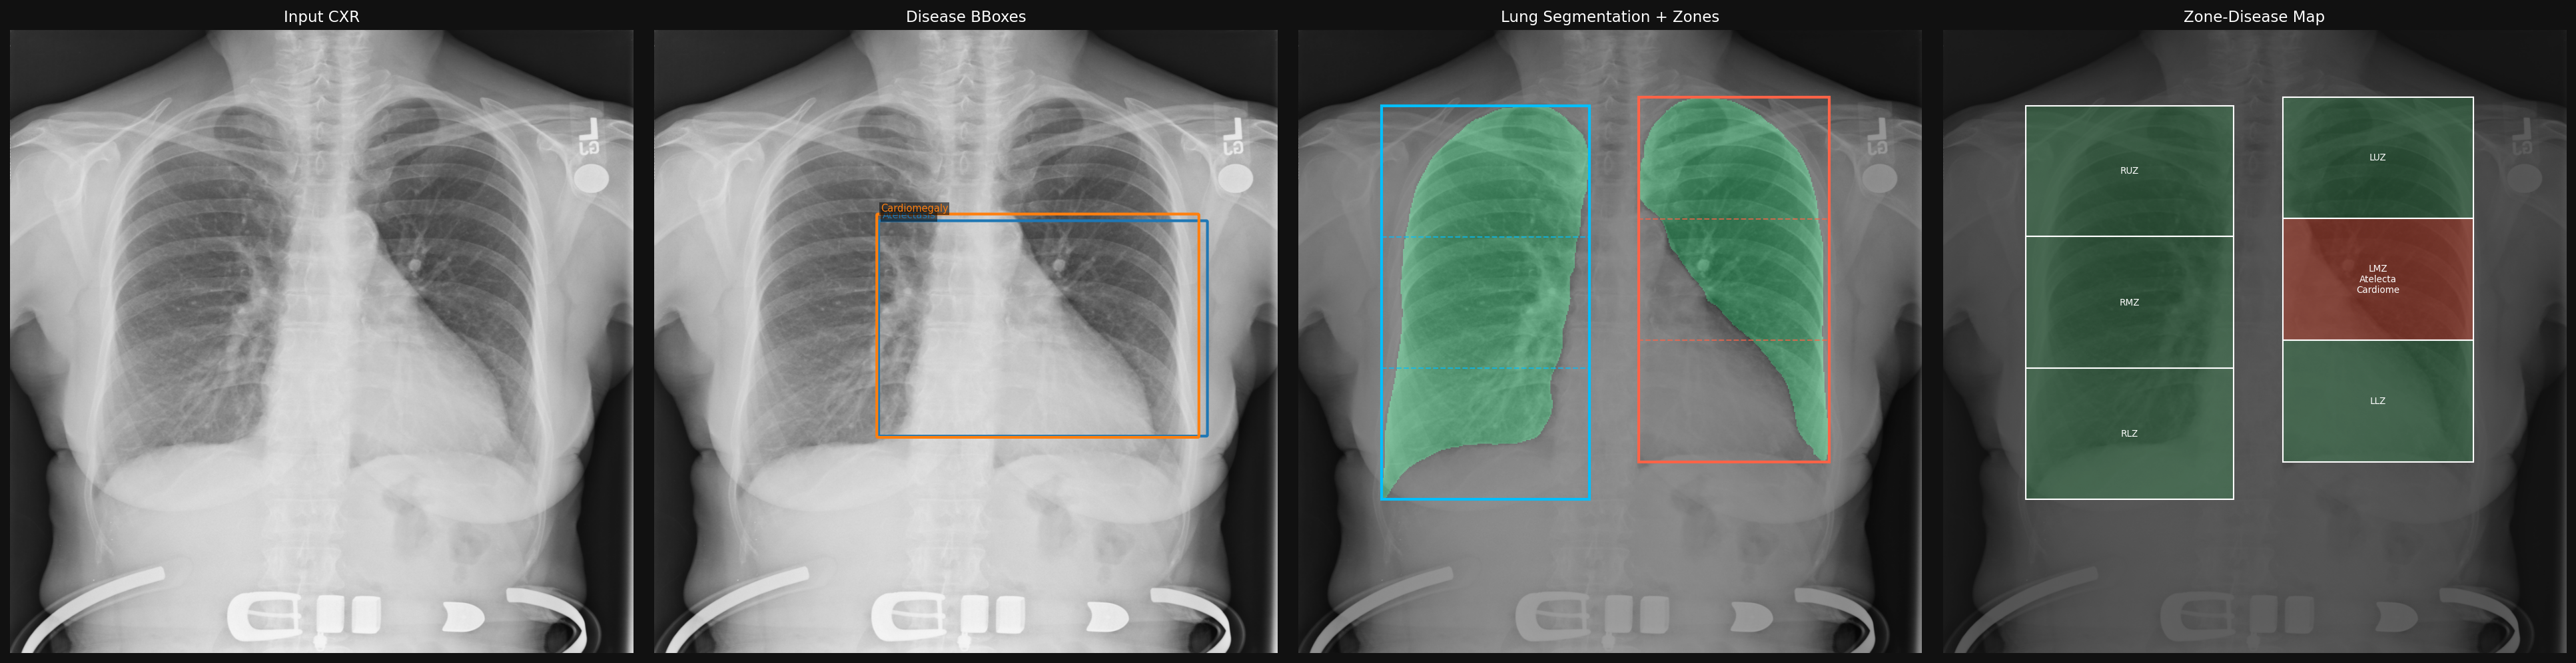
\includegraphics[width=\textwidth]{pipeline_result.png}
    \caption{End-to-end inference on a sample NIH chest radiograph: classification confidences, predicted bounding boxes, segmented lung fields, and the resulting zone-attributed structured report.}
    \label{fig:pipeline_viz}
\end{figure}
\FloatBarrier
%% ==================================================================
\section{Experimental Results}
\label{sec:results}
%% ==================================================================

\subsection{Performance Metrics}

Classification performance is reported using the area under the receiver-operating-characteristic curve (AUC-ROC), per class and as a macro-average across the 13 disease categories, together with macro- and micro-averaged F1 scores at both the default decision threshold (0.5) and after per-class threshold optimisation. Localisation performance is reported using Intersection over Union (IoU), both as a mean over the validation set and as the proportion of predictions exceeding IoU thresholds of 0.25 and 0.50. Segmentation performance is reported using the Dice coefficient, IoU (Jaccard index), and Boundary F1 (BF1), the latter capturing the precision of predicted lung-field contours.

\subsection{Multi-Label Classification Results}

The multimodal EfficientNet-B3 classifier was trained for up to 50 epochs with early stopping (patience~5), terminating at epoch~26 after validation AUC plateaued at \textbf{0.8636}. At the final recorded epoch, training metrics were Loss~0.0132, AUC~0.9198, F1~0.4777, while validation metrics were Loss~0.0172, AUC~0.8617, F1~0.3819; the resulting train--validation AUC gap of $\sim$0.058 indicates moderate overfitting that early stopping successfully contained (Figure~\ref{fig:learning_curves}).
\FloatBarrier
\begin{figure}[ht]
    \centering
    \begin{subfigure}[b]{0.48\textwidth}
        \centering
        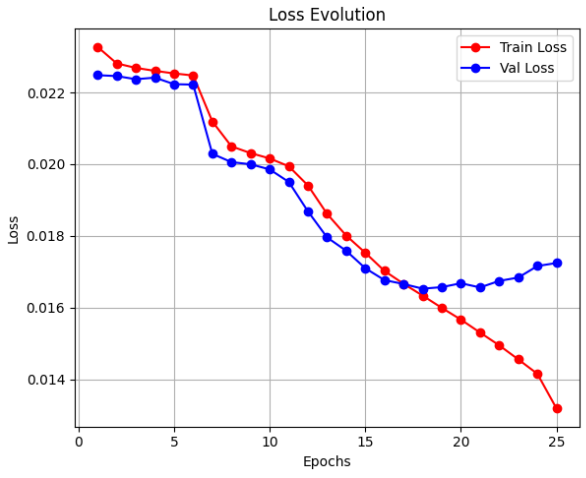
\includegraphics[width=\textwidth]{loss_auc_evolution.png}
        \caption{Training and validation loss.}
    \end{subfigure}
    \hfill
    \begin{subfigure}[b]{0.48\textwidth}
        \centering
        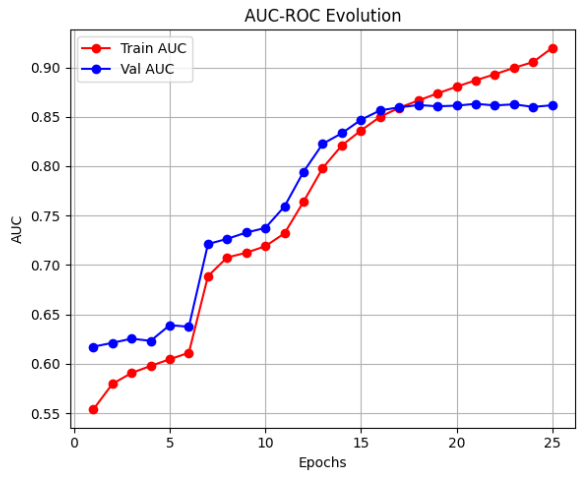
\includegraphics[width=\textwidth]{auc_with_control_line.png}
        \caption{AUC vs.\ epochs.}
    \end{subfigure}
    \caption{Learning curves for the supervised multimodal classifier.}
    \label{fig:learning_curves}
\end{figure}
\FloatBarrier
Table~\ref{tab:per_class_auc} reports per-class AUC-ROC on the validation set. Radiologically distinct pathologies with characteristic global appearance -- Emphysema (0.9714), Edema (0.9632), Fibrosis (0.9403), Pleural Thickening (0.9350), and Consolidation (0.9301) -- achieve excellent discrimination (AUC~$>0.93$). Diffuse or subtle findings such as Infiltration (0.7011), Nodule (0.7538), and Atelectasis (0.7817) remain more challenging, consistent with their well-documented inter-observer variability in the wider literature on NIH ChestX-ray14.

\begin{table}[ht]
\centering
\caption{Per-class AUC-ROC on the validation set.}
\label{tab:per_class_auc}
\renewcommand{\arraystretch}{1.2}
\begin{tabular}{lcc}
\toprule
\textbf{Pathology} & \textbf{AUC-ROC} & \textbf{Band} \\
\midrule
Emphysema           & 0.9714 & Excellent \\
Edema               & 0.9632 & Excellent \\
Fibrosis            & 0.9403 & Excellent \\
Pleural Thickening  & 0.9350 & Excellent \\
Consolidation       & 0.9301 & Excellent \\
Pneumonia           & 0.8981 & Good \\
Cardiomegaly        & 0.8824 & Good \\
Pneumothorax        & 0.8729 & Good \\
Effusion            & 0.8059 & Good \\
Mass                & 0.7907 & Moderate \\
Atelectasis         & 0.7817 & Moderate \\
Nodule              & 0.7538 & Moderate \\
Infiltration        & 0.7011 & Moderate \\
\midrule
\textbf{Overall mean} & \textbf{0.8636} & \textbf{Good} \\
\bottomrule
\end{tabular}
\end{table}

\subsection{Per-Class Threshold Optimisation}
\label{sec:threshold}

The default decision threshold of 0.5 is suboptimal for an imbalanced multi-label problem trained with Focal Loss, which systematically down-weights confident positive predictions. A per-class threshold search over $[0.0, 1.0]$ in steps of 0.01 was performed on the validation set to maximise per-class F1. As shown in Table~\ref{tab:threshold_overall}, this yields an improvement of $+0.166$ in macro-F1 (from 0.3444 to 0.5103) and $+0.103$ in micro-F1 (from 0.4232 to 0.5258), with a mean optimal threshold of 0.393.

\begin{table}[ht]
\centering
\caption{Overall F1 improvement from per-class threshold optimisation.}
\label{tab:threshold_overall}
\renewcommand{\arraystretch}{1.2}
\begin{tabular}{lccc}
\toprule
\textbf{Metric} & \textbf{Default (0.5)} & \textbf{Optimised} & \textbf{Improvement} \\
\midrule
Macro F1 & 0.3444 & 0.5103 & $+0.1660$ \\
Micro F1 & 0.4232 & 0.5258 & $+0.1026$ \\
\bottomrule
\end{tabular}
\end{table}

Table~\ref{tab:threshold_perclass} shows that the largest gains occur for classes that were entirely suppressed at the default threshold: Fibrosis ($+0.397$) and Pneumonia ($+0.240$) had zero F1 at threshold~0.5 due to their low positive sample counts (408 and 328 respectively) and only become detectable once the threshold is lowered. Pleural Thickening ($+0.317$) and Nodule ($+0.237$) also improve substantially. The smallest gains are observed for already well-performing classes such as Effusion ($+0.035$) and Emphysema ($+0.037$). Figure~\ref{fig:threshold_opt} visualises the distribution of optimal thresholds, which is concentrated in $[0.32, 0.44]$, well below the default of 0.5.

\begin{table}[ht]
\centering
\caption{Per-class threshold optimisation results.}
\label{tab:threshold_perclass}
\renewcommand{\arraystretch}{1.2}
\begin{tabular}{lccccr}
\toprule
\textbf{Pathology} & \textbf{Def.\ Thr.} & \textbf{Opt.\ Thr.} & \textbf{Def.\ F1} & \textbf{Opt.\ F1} & \textbf{$\Delta$F1} \\
\midrule
Atelectasis         & 0.500 & 0.390 & 0.4377 & 0.5384 & $+0.1007$ \\
Cardiomegaly        & 0.500 & 0.370 & 0.4532 & 0.5373 & $+0.0840$ \\
Consolidation       & 0.500 & 0.400 & 0.3935 & 0.5715 & $+0.1780$ \\
Edema               & 0.500 & 0.400 & 0.3531 & 0.5806 & $+0.2275$ \\
Effusion            & 0.500 & 0.420 & 0.5573 & 0.5921 & $+0.0348$ \\
Emphysema           & 0.500 & 0.440 & 0.6441 & 0.6807 & $+0.0366$ \\
Fibrosis            & 0.500 & 0.350 & 0.0000 & 0.3973 & $+0.3973$ \\
Infiltration        & 0.500 & 0.410 & 0.4380 & 0.5327 & $+0.0947$ \\
Mass                & 0.500 & 0.400 & 0.2812 & 0.4531 & $+0.1719$ \\
Nodule              & 0.500 & 0.400 & 0.1872 & 0.4241 & $+0.2369$ \\
Pleural Thickening  & 0.500 & 0.390 & 0.1919 & 0.5085 & $+0.3166$ \\
Pneumonia           & 0.500 & 0.320 & 0.0000 & 0.2395 & $+0.2395$ \\
Pneumothorax        & 0.500 & 0.420 & 0.5393 & 0.5784 & $+0.0391$ \\
\midrule
\textbf{Average}    & 0.500 & \textbf{0.393} & 0.3444 & \textbf{0.5103} & \textbf{$+0.1660$} \\
\bottomrule
\end{tabular}
\end{table}
\FloatBarrier
\begin{figure}[ht]
    \centering
    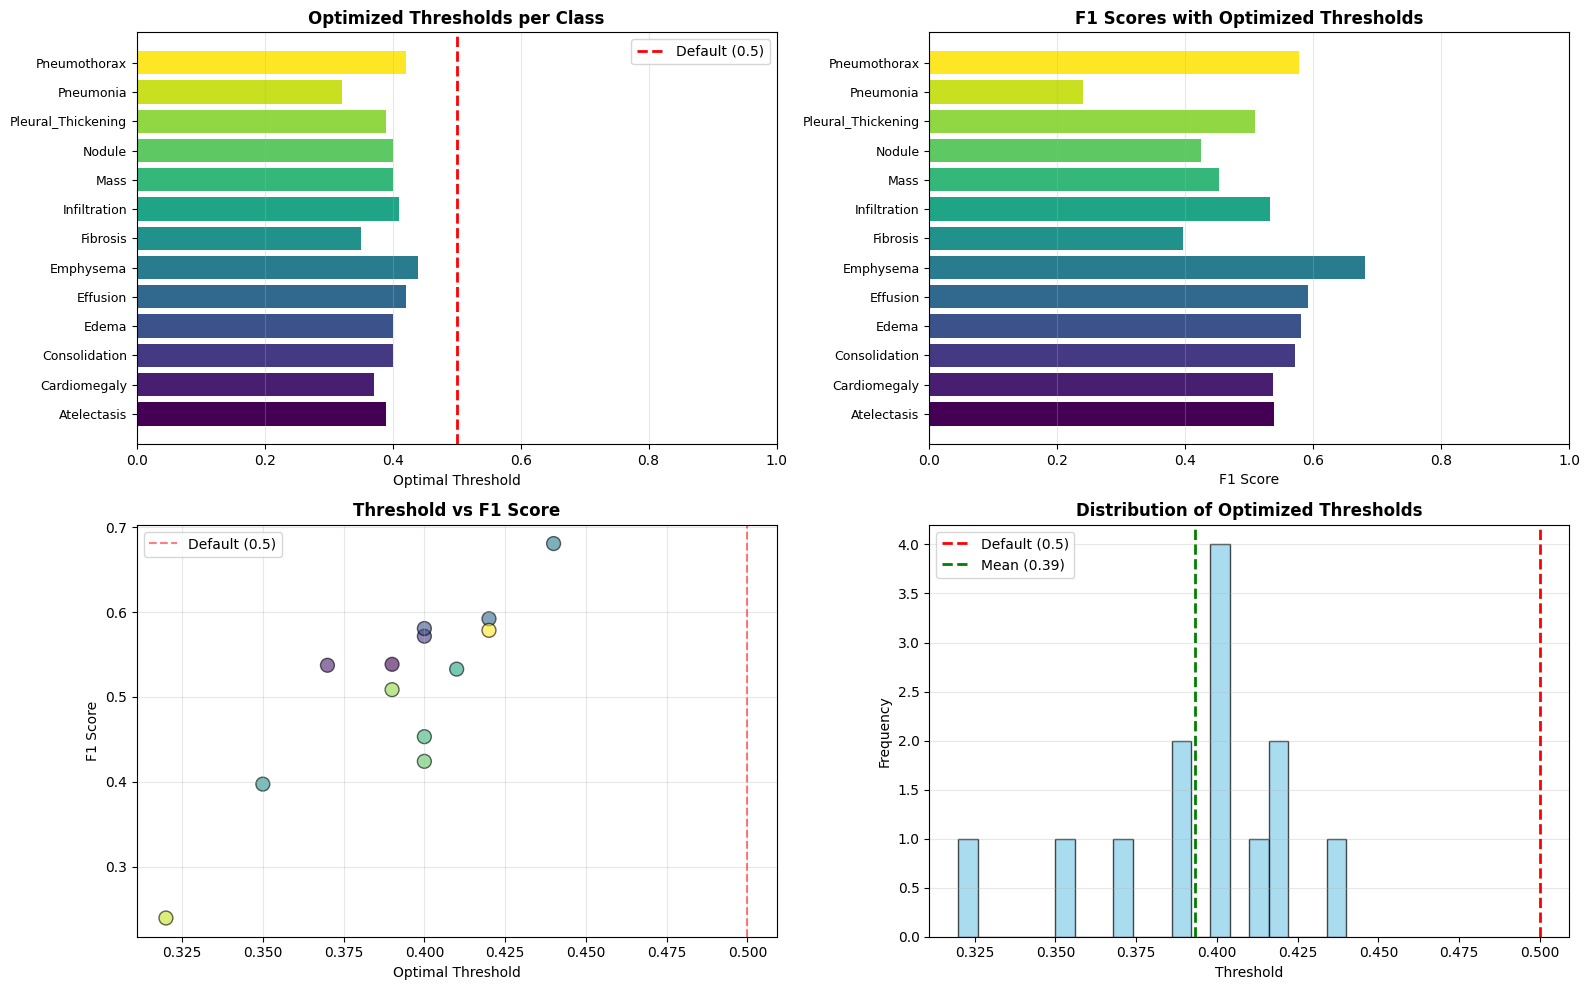
\includegraphics[width=0.95\textwidth]{threshold_optimization_results.png}
    \caption{Threshold optimisation results: (top-left) optimal thresholds per class, (top-right) F1 at optimised thresholds, (bottom-left) threshold vs.\ F1, (bottom-right) distribution of optimal thresholds.}
    \label{fig:threshold_opt}
\end{figure}
\FloatBarrier
\subsection{Representation Quality}

t-SNE projections of the learned EfficientNet-B3 embeddings (Figure~\ref{fig:tsne_per_disease}) show that radiologically distinct pathologies such as Emphysema, Cardiomegaly, and Edema form tight, well-separated clusters relative to normal cases, consistent with their high per-class AUC. Diffuse pathologies such as Infiltration and Atelectasis overlap more with the normal distribution, reflecting their inherent visual ambiguity. At a coarse level, the model separates any-disease from normal cases (Figure~\ref{fig:tsne_any_vs_normal}), indicating that the learned representation captures a global notion of anatomical normality.
\FloatBarrier
\begin{figure}[ht]
    \centering
    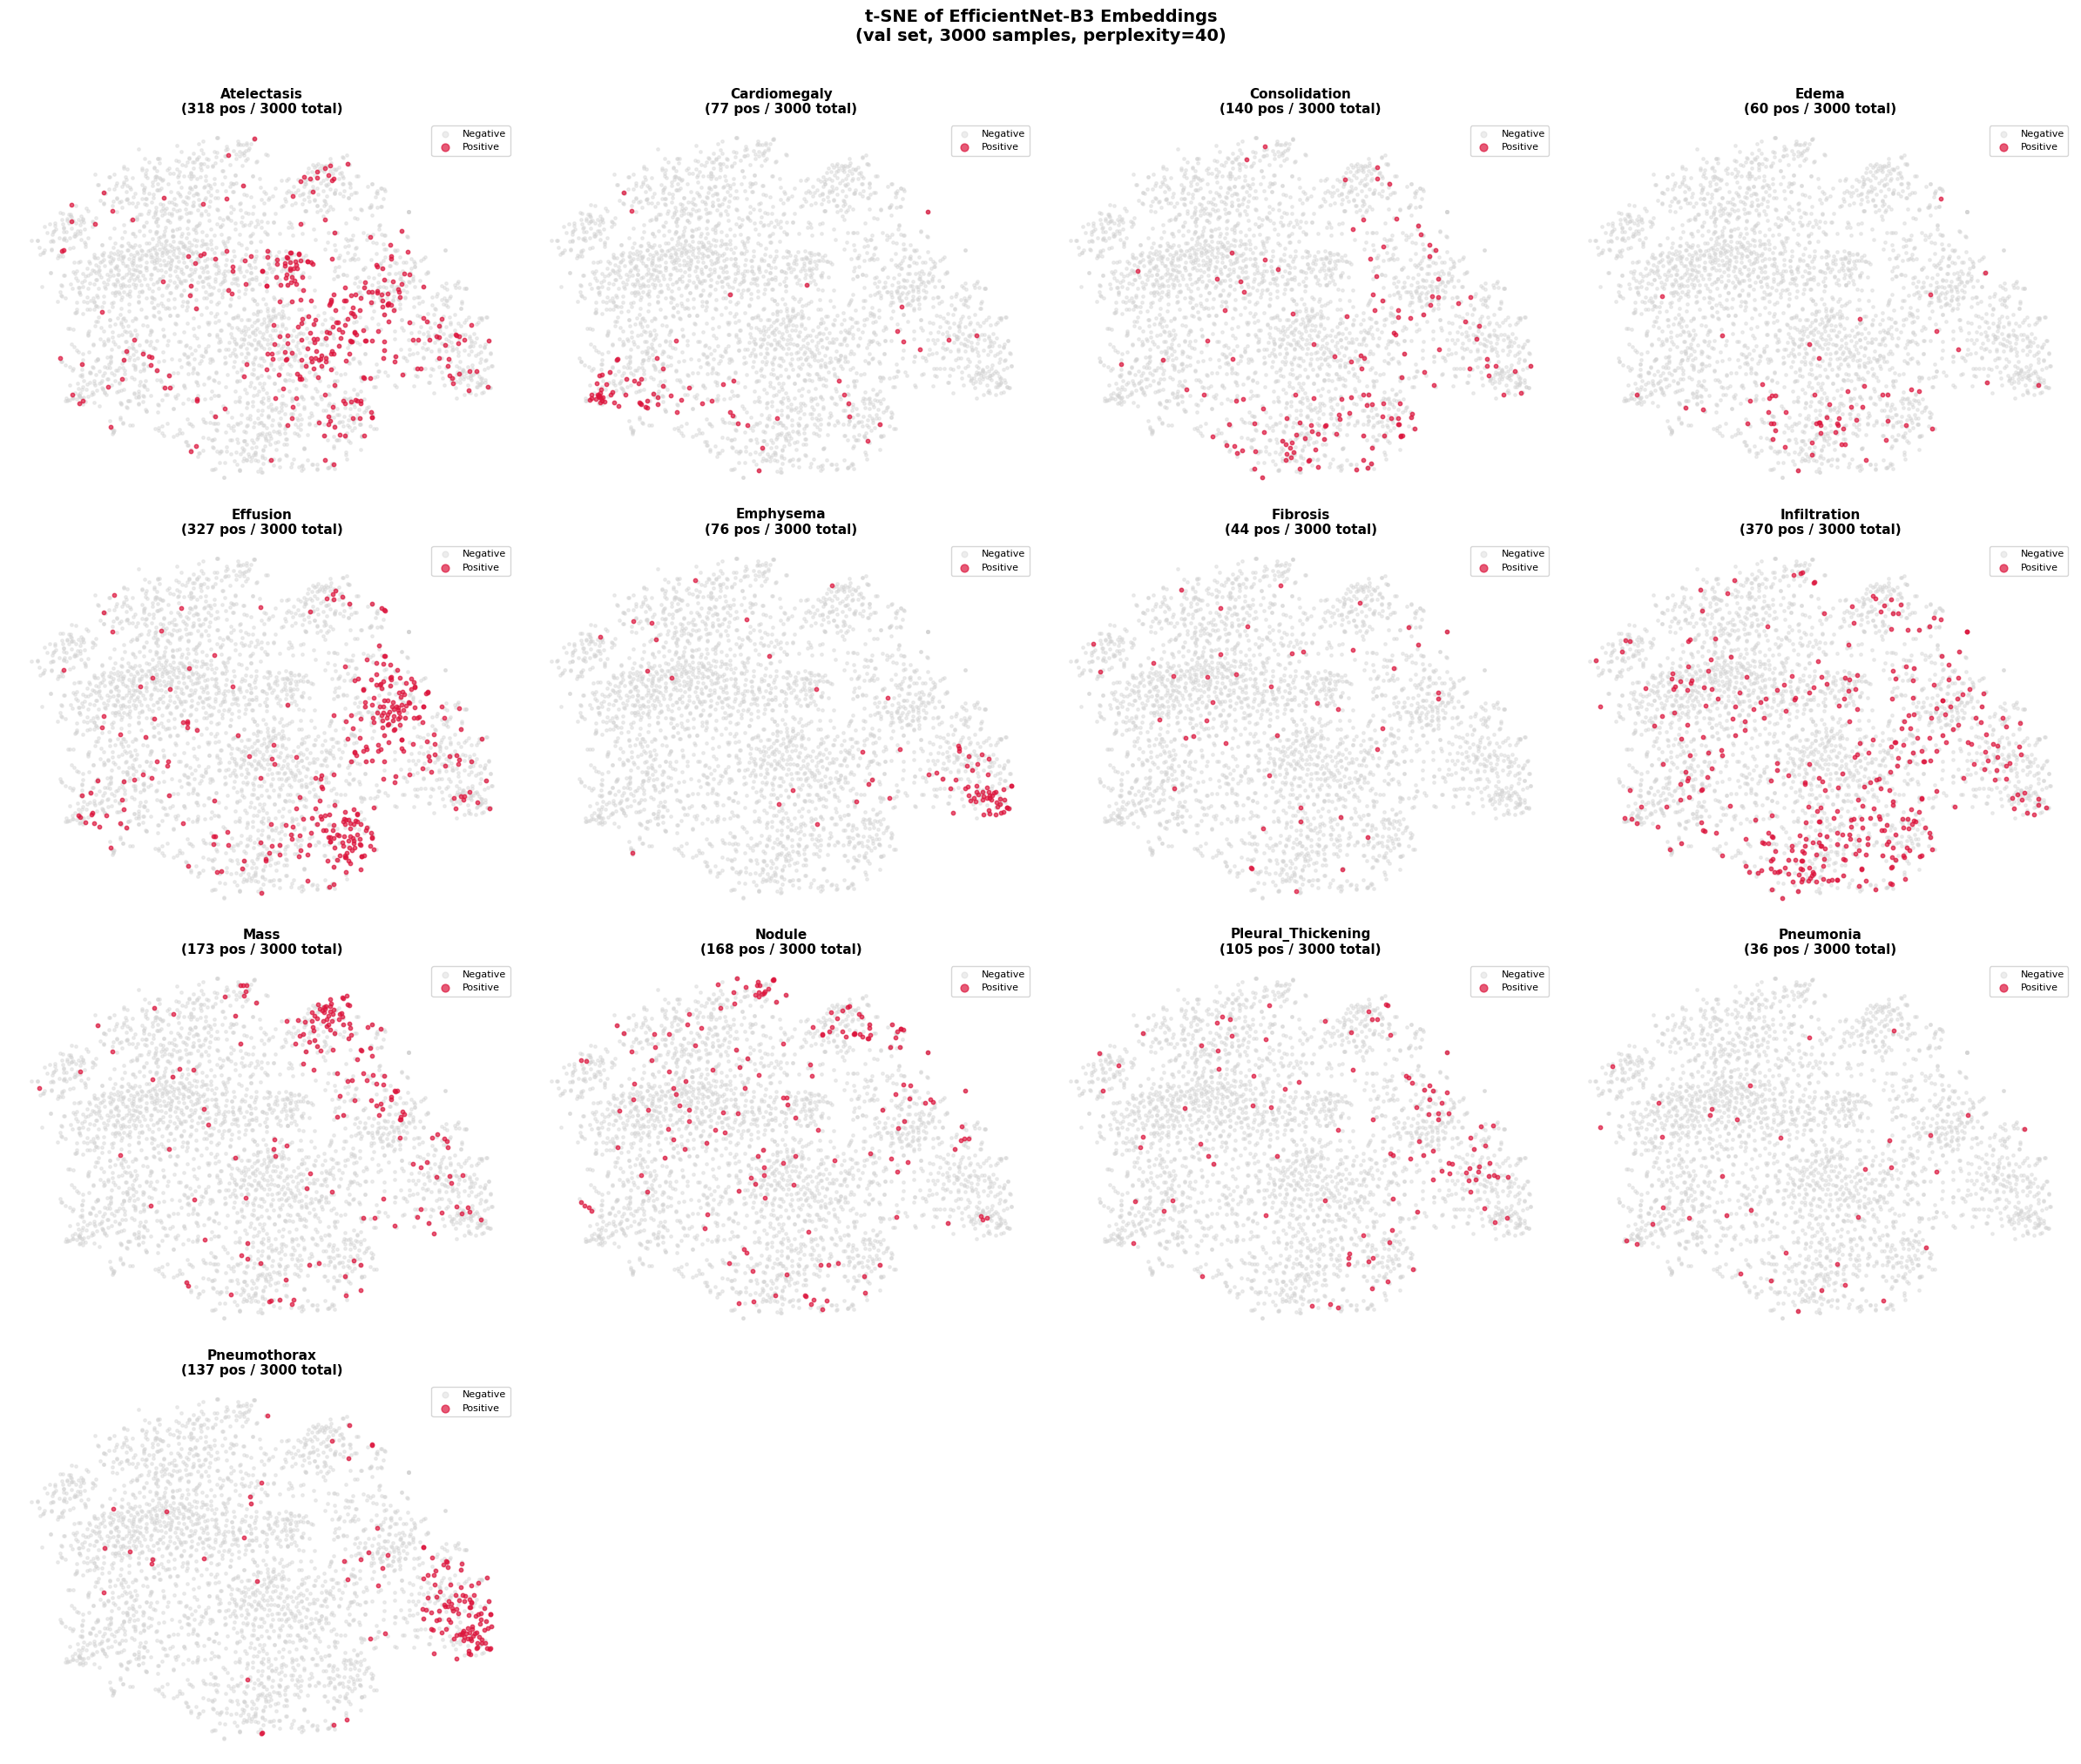
\includegraphics[width=0.85\textwidth]{tsne_disease_vs_normal.png}
    \caption{t-SNE projection of validation embeddings coloured by individual disease label versus Normal.}
    \label{fig:tsne_per_disease}
\end{figure}

\begin{figure}[ht]
    \centering
    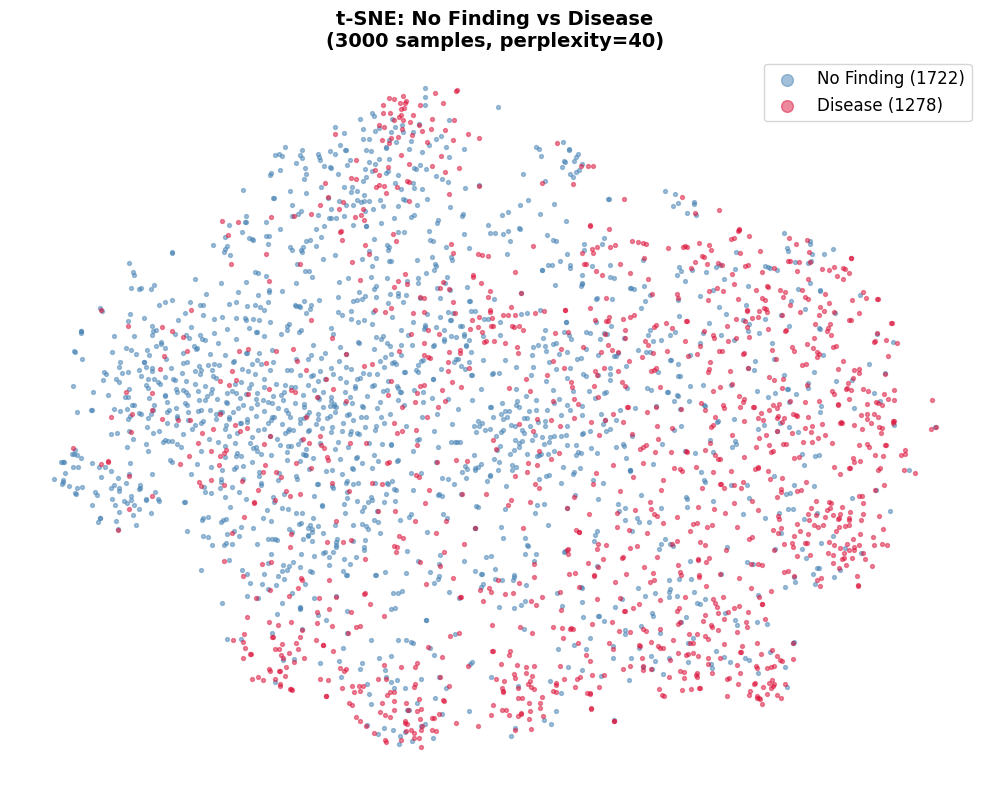
\includegraphics[width=0.55\textwidth]{tsne_anydisease_vs_normal.png}
    \caption{t-SNE projection coloured by any-disease-present versus Normal.}
    \label{fig:tsne_any_vs_normal}
\end{figure}
\FloatBarrier
\subsection{Disease Localisation Results}

The bounding-box regressor was trained for up to 60 epochs with early stopping (patience~8), halting at epoch~34 with a best validation mean IoU of \textbf{0.2110} (Table~\ref{tab:bbox_training}, Figure~\ref{fig:bbox_curves}). Table~\ref{tab:bbox_perclass} shows substantial per-class variation: Cardiomegaly achieves a mean IoU of 0.6607 and an IoU@0.50 hit-rate of 82.8\%, indicating near-clinical-grade localisation, consistent with its large, globally positioned, and radiologically unambiguous presentation. Effusion (0.154) and Pneumothorax (0.113) achieve partial localisation, while Atelectasis, Mass, and Nodule fail to reach IoU@0.50 for any sample, reflecting their small lesion size, positional variability, and the limited size of the NIH bounding-box annotation set (880 images across 8 classes). For comparison, localisation models trained on the larger, radiologist-annotated VinBigData chest X-ray dataset typically reach mean IoU in the range 0.45--0.55, suggesting that the overall mean IoU reported here is limited primarily by annotation scale rather than representation quality.

\begin{table}[ht]
\centering
\caption{Bounding-box regression summary at early stopping (epoch 34).}
\label{tab:bbox_training}
\renewcommand{\arraystretch}{1.2}
\begin{tabular}{lcccc}
\toprule
\textbf{Split} & \textbf{Loss} & \textbf{mIoU} & \textbf{IoU@0.25} & \textbf{IoU@0.50} \\
\midrule
Train & 0.7518 & 0.3056 & 0.466 & 0.270 \\
Val   & 0.9392 & 0.2063 & 0.336 & 0.161 \\
\bottomrule
\end{tabular}
\end{table}
\FloatBarrier
\begin{figure}[ht]
    \centering
    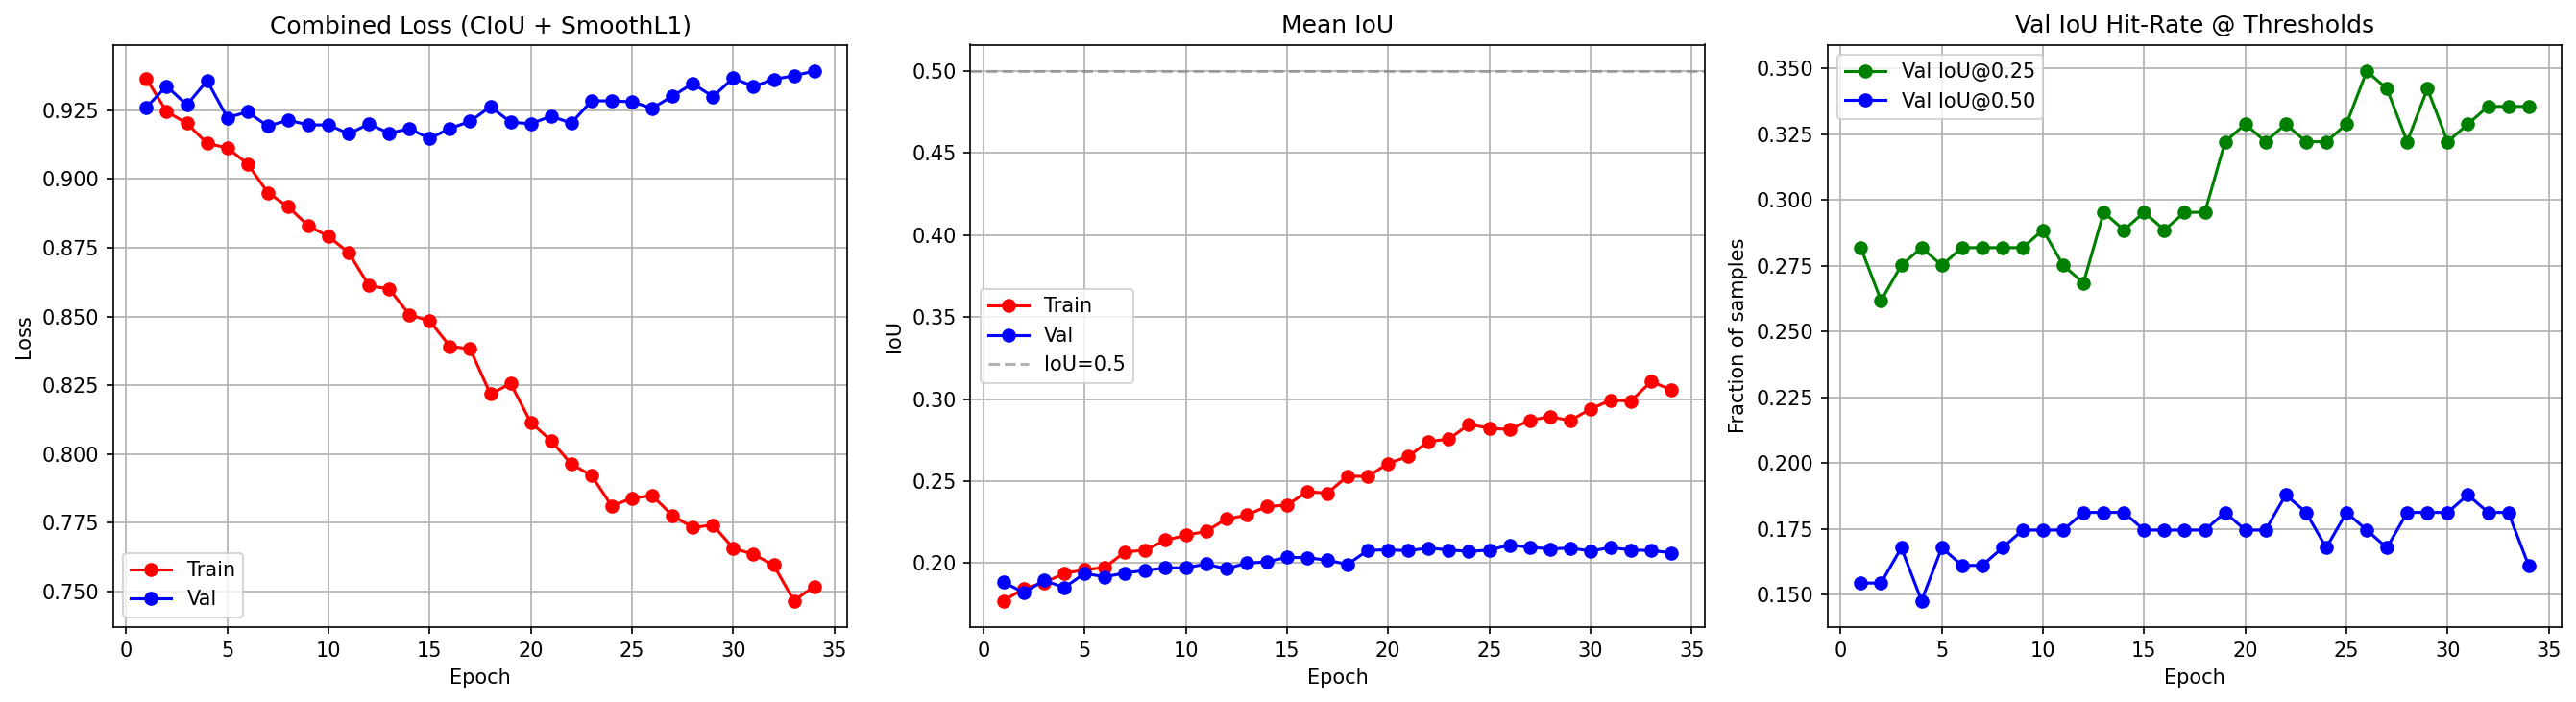
\includegraphics[width=\textwidth]{bbox_training_curves.png}
    \caption{Bounding-box regression training curves: (left) CIoU + Smooth-L1 loss, (centre) mean IoU, (right) validation IoU hit-rate at 0.25 and 0.50.}
    \label{fig:bbox_curves}
\end{figure}
\FloatBarrier
\begin{table}[ht]
\centering
\caption{Per-class IoU on the bounding-box validation set.}
\label{tab:bbox_perclass}
\renewcommand{\arraystretch}{1.2}
\begin{tabular}{lccc}
\toprule
\textbf{Disease} & \textbf{\# Samples} & \textbf{Mean IoU} & \textbf{IoU@0.50} \\
\midrule
Cardiomegaly  & 29  & \textbf{0.6607} & \textbf{0.828} \\
Effusion      & 31  & 0.1540 & 0.032 \\
Pneumothorax  & 20  & 0.1125 & 0.050 \\
Atelectasis   & 36  & 0.0909 & 0.000 \\
Mass          & 17  & 0.1032 & 0.000 \\
Nodule        & 16  & 0.0143 & 0.000 \\
\midrule
\textbf{Overall} & \textbf{149} & \textbf{0.2110} & \textbf{0.174} \\
\bottomrule
\end{tabular}
\end{table}
\FloatBarrier
\begin{figure}[ht]
    \centering
    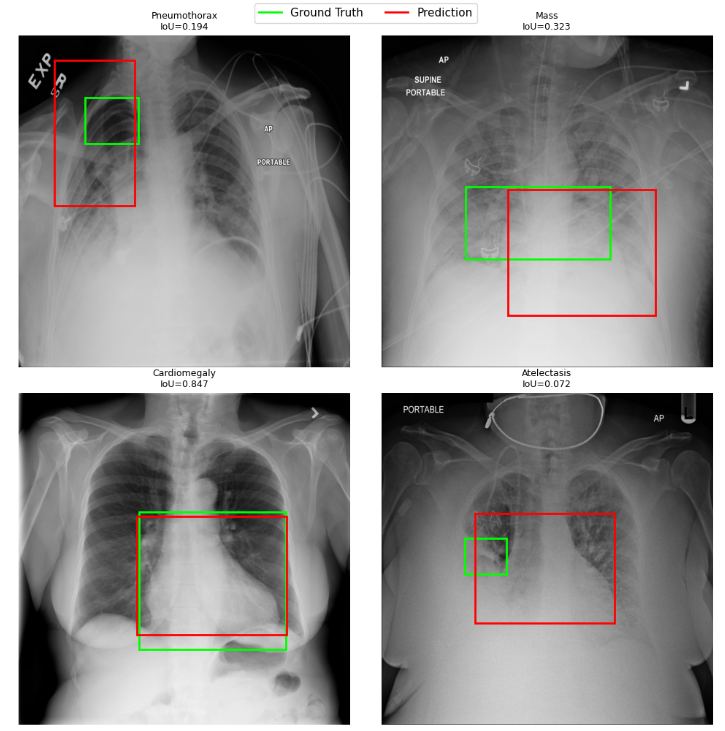
\includegraphics[width=0.75\textwidth]{bbox_predictions_viz.png}
    \caption{Qualitative bounding-box predictions on the validation set (green: ground truth, red: prediction); per-sample IoU is shown in each subplot title.}
    \label{fig:bbox_viz}
\end{figure}
\FloatBarrier
\subsection{Lung Segmentation Results}

The edge-aware U-Net was trained for the full 60 epochs without early stopping, reaching a Dice coefficient of \textbf{0.9602}, an IoU of \textbf{0.9249}, and a Boundary F1 of \textbf{0.7246} at the final epoch (Table~\ref{tab:segmentation}, Figure~\ref{fig:seg_curves}). The high Dice and IoU indicate near-perfect overall lung-field delineation, while the more modest Boundary F1 reflects the difficulty of precisely tracing fine contours near the cardiac silhouette and diaphragm -- the region targeted by the boundary-weighted BCE and auxiliary edge head. Figure~\ref{fig:seg_viz} shows a qualitative example, including the bounding boxes used for the zone-division step described in Section~\ref{sec:report-gen}.

\begin{table}[ht]
\centering
\caption{Lung segmentation performance at epoch 60 on the validation set.}
\label{tab:segmentation}
\renewcommand{\arraystretch}{1.2}
\begin{tabular}{lc}
\toprule
\textbf{Metric} & \textbf{Score} \\
\midrule
Dice Coefficient   & 0.9602 \\
IoU (Jaccard)      & 0.9249 \\
Boundary F1 (BF1)  & 0.7246 \\
Train Loss         & 0.4671 \\
Val Loss           & 0.4633 \\
\bottomrule
\end{tabular}
\end{table}
\FloatBarrier
\begin{figure}[ht]
    \centering
    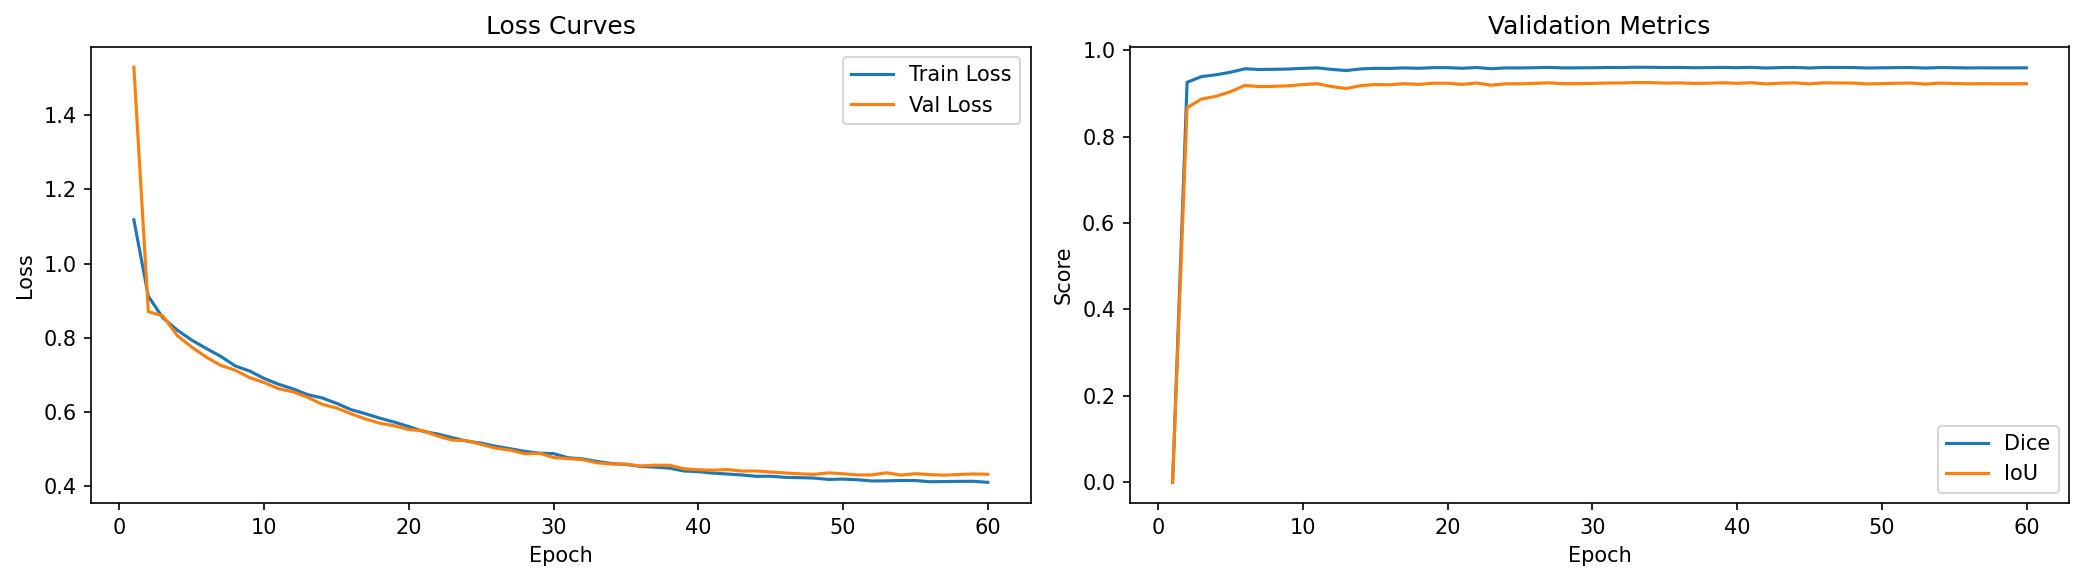
\includegraphics[width=\textwidth]{training_curves.png}
    \caption{Segmentation training curves: combined loss (train/validation) and validation Dice, IoU, and Boundary F1 over 60 epochs.}
    \label{fig:seg_curves}
\end{figure}
\begin{figure}[ht]
    \centering
    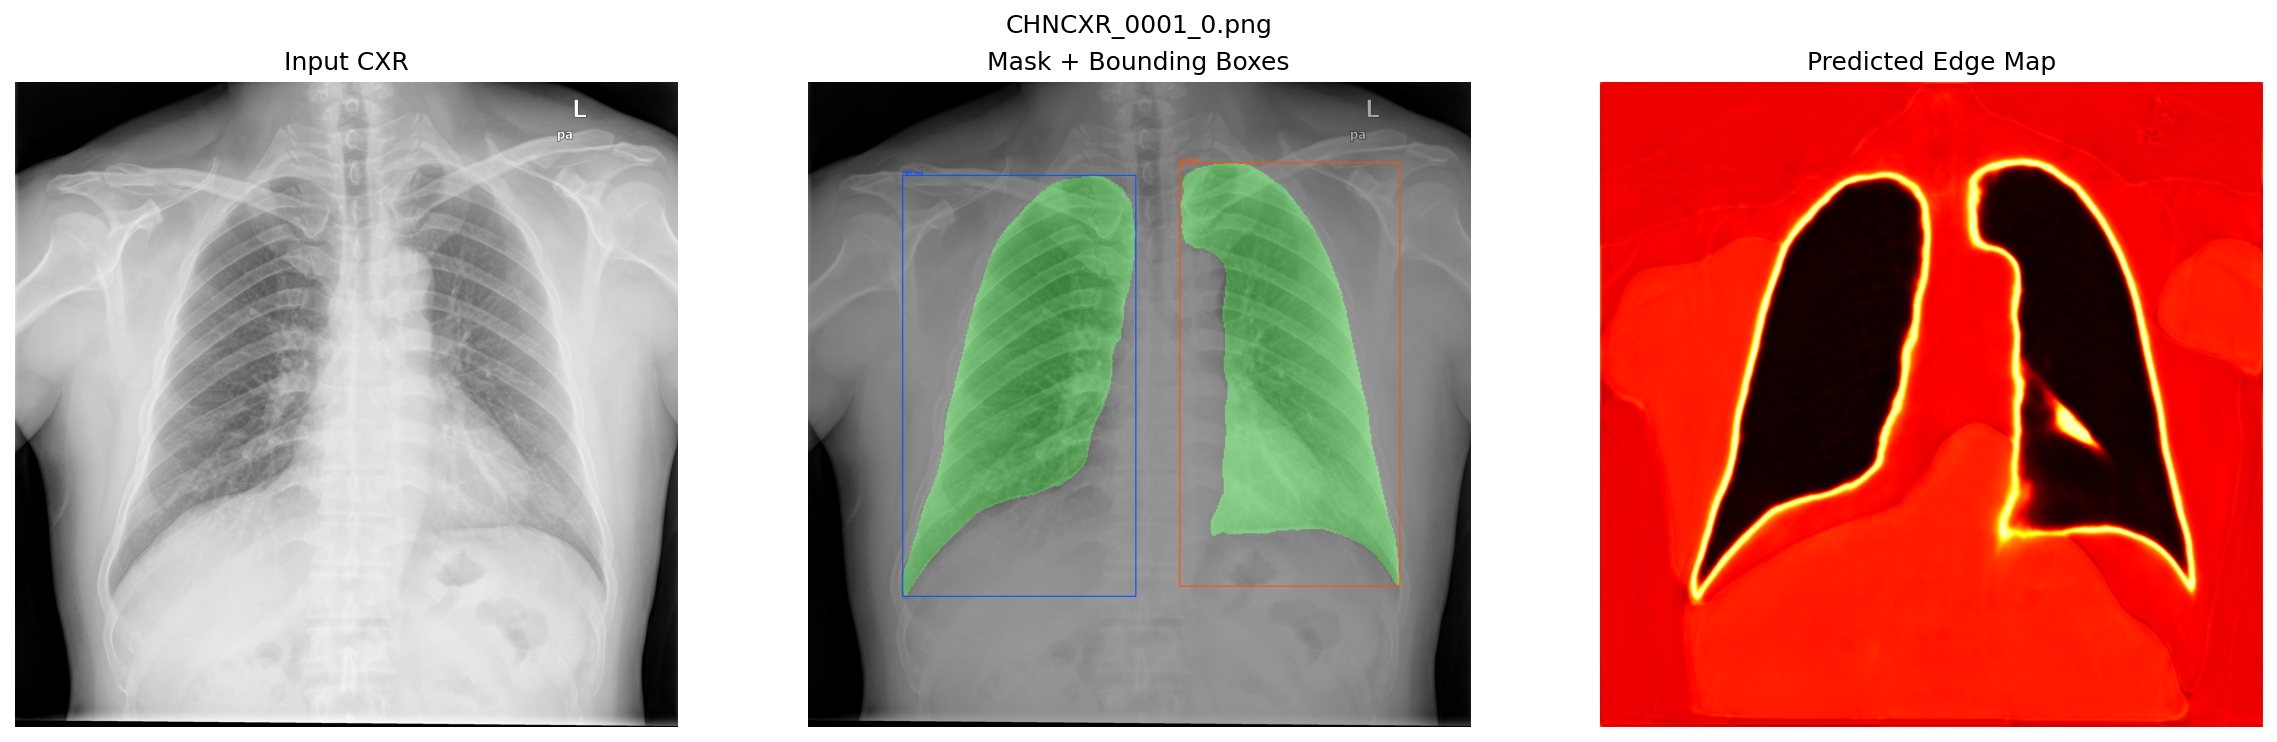
\includegraphics[width=0.7\textwidth]{sample_prediction.png}
    \caption{Qualitative segmentation output: predicted binary lung mask overlaid on the input radiograph, with the left/right lung bounding boxes used for zone division.}
    \label{fig:seg_viz}
\end{figure}
\FloatBarrier
\subsection{Note on Self-Supervised Pre-Training}
\label{sec:ssl-results}

The exploratory self-supervised pre-training stage (Section~\ref{sec:ssl}) converged smoothly over three epochs, with the composite loss $\mathcal{L}_{\text{SSL}}$ falling from 1.7447 (epoch~1) to 0.4308 (epoch~2) and 0.2672 (epoch~3), indicating that the optimal-transport alignment, variance, and covariance terms jointly drive the backbone toward a compact, decorrelated representation of chest-radiograph patches. However, when this pre-trained backbone was used to initialise the supervised classifier and evaluated under varying labelled-data fractions (Table~\ref{tab:label_efficiency}), the resulting (SL+SSL) model matched the supervised-only (SL) baseline at 100\% and 50\% of labels (0.8636 vs.\ $\sim$0.860, and 0.8608 vs.\ $\sim$0.860, respectively), but \emph{underperformed} the supervised-only model at 25\% of labels (0.8271 vs.\ $\sim$0.850) and showed no clear advantage at 10\%. This suggests that, in its current form, the patch-level optimal-transport objective over-specifies the representation for structural alignment at the expense of fine-grained class discriminability when labels are scarce. Given these mixed results, the SSL stage is not recommended as a default component of the pipeline; it is retained here only as a documented exploratory finding and as motivation for the future-work directions discussed in Section~\ref{sec:conclusion}.

\begin{table}[ht]
\centering
\caption{Mean AUC-ROC at varying labelled-data fractions, supervised-only (SL) vs.\ SSL-pretrained (SL+SSL).}
\label{tab:label_efficiency}
\renewcommand{\arraystretch}{1.2}
\begin{tabular}{lcc}
\toprule
\textbf{Labelled Data Fraction} & \textbf{SL only} & \textbf{SL + SSL} \\
\midrule
100\% & $\sim$0.860 & 0.8636 \\
50\%  & $\sim$0.860 & 0.8608 \\
25\%  & $\sim$0.850 & 0.8271 \\
10\%  & $\sim$0.830--0.840 & $>$0.80 \\
\bottomrule
\end{tabular}
\end{table}

%% ==================================================================
\section{Comparison with State of the Art}
\label{sec:comparison}
%% ==================================================================

\subsection{Comparison with Supervised Baselines on NIH ChestX-ray14}

To contextualise the contribution of the multimodal architecture, the proposed model is compared against several baseline architectures trained under the same supervised protocol and data split (Table~\ref{tab:baselines}). ResNet-50 and DenseNet-121 serve as lightweight CNN references, while a ViT/Swin Transformer baseline represents a transformer-based alternative. The proposed multimodal EfficientNet-B3 classifier (with metadata fusion and Focal Loss) achieves the highest mean AUC-ROC of 0.8636, an improvement of $+0.0136$ over the equivalent EfficientNet-B3 model without metadata fusion or SSL pre-training (0.85), and substantially ahead of DenseNet-121 (0.77) and ResNet-50 (0.60). The ViT/Swin baseline (0.80, after 7 epochs with partially frozen layers) suggests that transformer-based backbones require longer fine-tuning schedules to become competitive on this dataset.
\FloatBarrier
\begin{table}[ht]
\centering
\caption{Comparison of mean AUC-ROC across baseline architectures and the proposed model on NIH ChestX-ray14.}
\label{tab:baselines}
\renewcommand{\arraystretch}{1.3}
\begin{tabular}{lcl}
\toprule
\textbf{Model} & \textbf{Mean AUC-ROC} & \textbf{Notes} \\
\midrule
ResNet-50 (supervised)        & 0.60 & Fully supervised, no metadata fusion \\
DenseNet-121 (supervised)     & 0.77 & Fully supervised, no metadata fusion \\
ViT / Swin Transformer        & 0.80 & After 7 epochs, partially frozen \\
EfficientNet-B3 (supervised)  & 0.85 & Multimodal, no SSL pre-training \\
\rowcolor{gray!15}
\textbf{Proposed:} & \textbf{0.8636} & Best result \\
\bottomrule
\end{tabular}
\end{table}
\FloatBarrier
\subsection{Qualitative Comparison with the Report-Generation Literature}

A direct numerical comparison with the report-generation literature reviewed in Section~\ref{sec:litreview} is not straightforward, because those works typically report language-generation metrics (BLEU, ROUGE) on MIMIC-CXR or IU-XRAY \citep{yang_knowledge,mmg_fusion}, whereas the present work reports classification AUC/F1, localisation IoU, and segmentation Dice/IoU on NIH ChestX-ray14 and the Shenzhen dataset. Table~\ref{tab:qualitative_comparison} therefore provides a qualitative comparison along the dimensions identified in Section~\ref{sec:gaps}: spatial grounding, use of patient metadata, modularity, and structured (zone-attributed) output.

\begin{table}[ht]
\centering
\caption{Qualitative comparison with representative literature approaches.}
\label{tab:qualitative_comparison}
\renewcommand{\arraystretch}{1.3}
\begin{tabular}{p{3.0cm}p{2.0cm}p{2.0cm}p{2.0cm}p{3.0cm}}
\toprule
\textbf{Approach} & \textbf{Spatial Grounding} & \textbf{Metadata Fusion} & \textbf{Modular} & \textbf{Structured / Zonal Output} \\
\midrule
\citet{yang_knowledge} & No & No & No (end-to-end) & No \\
\citet{mmg_fusion} & Partial (multi-scale features) & Patient history (text) & Partial & No \\
\citet{ihras} & Yes (Grad-CAM + segmentation) & Not specified & Yes & Limited \\
\citet{xrem} & No & No & Yes (retrieval) & No \\
\citet{concept_rag} & Concept-level & No & Yes & Concept bottleneck \\
\textbf{Proposed} & \textbf{Yes (bbox + segmentation)} & \textbf{Yes (age, sex, view)} & \textbf{Yes} & \textbf{Yes (6-zone report)} \\
\bottomrule
\end{tabular}
\end{table}

Relative to these approaches, the proposed pipeline is the only one in this comparison that combines quantitatively evaluated bounding-box localisation, lung-field segmentation, patient-metadata fusion, and an automatically generated zone-attributed structured report within a single system evaluated on a large public dataset.

%% ==================================================================
\section{Conclusion and Future Work}
\label{sec:conclusion}
%% ==================================================================

This paper presented a multimodal, modular pipeline for automated chest X-ray analysis built around an EfficientNet-B3 backbone. A multimodal classifier that fuses image features with patient age, sex, and view-position metadata, trained with a multi-label Focal Loss, achieved a mean AUC-ROC of 0.8636 across 13 thoracic disease categories on the NIH ChestX-ray14 dataset, outperforming ResNet-50 (0.60), DenseNet-121 (0.77), a ViT/Swin baseline (0.80), and an EfficientNet-B3 model without metadata fusion (0.85). Per-class threshold optimisation improved macro-F1 from 0.3444 to 0.5103, with the largest gains for previously suppressed rare classes such as Fibrosis and Pneumonia. A disease-conditioned bounding-box regressor reached a mean IoU of 0.2110 on the NIH BBox\_List\_2017 subset, with near-clinical localisation for cardiomegaly (IoU 0.6607, IoU@0.50 82.8\%), and an edge-aware U-Net achieved a Dice coefficient of 0.9602 for lung-field segmentation on the Shenzhen dataset. These three modules were combined into a zone-based, template-driven report generator that attributes detected pathologies to one of six anatomical zones. An exploratory optimal-transport-inspired self-supervised pre-training stage was also evaluated; it produced only a marginal change in overall AUC and was not consistently beneficial at reduced label fractions, and is therefore reported as a secondary, exploratory finding rather than a core contribution.

Several directions for future work follow directly from these results. First, the disease-localisation module is currently constrained by the small NIH bounding-box annotation set (880 images); fine-tuning on the larger, radiologist-annotated VinBigData chest X-ray dataset is expected to raise mean IoU from 0.2110 toward the 0.45--0.55 range typically reported on that dataset, with no architectural changes required. Second, the boundary precision of the segmentation module (BF1 0.7246) could be improved with a larger or more diverse segmentation training corpus and lobe-aware (rather than purely horizontal) zone division, improving the anatomical precision of zone-to-disease attribution. Third, the current report generator is template-driven; integrating a vision--language model fine-tuned on MIMIC-CXR reports as a drafting head -- conditioned on the detected diseases, their zones, and the segmentation outputs -- would allow the pipeline to generate free-form, radiologist-style findings and impressions, building on the retrieval-augmented and concept-bottleneck approaches discussed in Section~\ref{sec:litreview} \citep{xrem,concept_rag}. Finally, the mixed results of the exploratory self-supervised pre-training stage (Section~\ref{sec:ssl-results}) suggest that future work should investigate objectives that more directly bridge patch-level structural alignment with class-level discriminability -- for example via pseudo-label consistency regularisation during fine-tuning, longer pre-training schedules, curriculum-based fine-tuning, or expanding the pre-training corpus to include CheXpert, MIMIC-CXR, or PadChest -- before such pre-training is adopted as a default component of the pipeline.

%% ==================================================================
% Bibliography
%% ==================================================================

\bibliographystyle{elsarticle-harv}
\bibliography{References}

\end{document}
%%
%% End of file.